\chapter{The Effects of Vegetation Density Upon Flow and Mass Transport in Lateral Cavities}
\label{chap:art4}
In this chapter, the main topic of this dissertation is developed. The effects of vegetation on the hydrodynamics and the mass exchange between the main channel/dead zone are investigated. The objective of this paper was to describe and possibly find a threshold on the behaviour of the dead zone given a certain density level.

\section*{Authors}
\begin{itemize}
    \item Luiz Eduardo Domingos de Oliveira \footnote{Federal University of Mato Grosso do Sul}
    \item Taís Natsumi Yamasaki \footnotemark[1]
    \item Filipe de Lima Queiroz \footnotemark[1]
    \item Felipe Rezende da Costa \footnotemark[1]
    \item Johannes Gérson Janzen \footnotemark[1]
    \item Carlo Gualtieri \footnote{University of Naples Federico II}
\end{itemize}

\addcontentsline{toc}{section}{Abstract}
\section*{Abstract}
Lateral cavities are regions attached to rivers affect the flow by creating a dead water zone. These regions reduce the flow velocity increasing the deposition of sediment and the temporary storage of polluted materials, which favours the growth of aquatic vegetation. The effect of this vegetation growth was studied using different vegetation densities in a Large Eddy Simulation (LES). The vegetation drag was represented by a porous media calculated with the Darcy-Forchheimer model. This numerical model showed that the hydrodynamics of the flow can present different patterns and phases for a vegetation density $0<a(\%)<10.656$. Furthermore, the occurrence of a secondary circulation was found where it normally would not occur for a non-vegetated scenario.

\noindent\textbf{Keywords:}: Lateral Cavity; Aquatic Vegetation; Mass Exchange; Computational Fluid Dynamics (CFD).

\section{Introduction}
Lateral cavities are an important component of riverine \cite{Harvey2015} and estuarine \cite{Ward1984} systems, because they (1) function as a macro-roughness at the river banks \cite{juez2017}, (2) drive mass exchange processes with the open channel \cite{Ouro2020, Mignot2017,jackson2015}, (3) act as transient storage zones \cite{jackson2015,drost2014,jackson2013a}, and (4) enhance biodiversity in the system \cite{harvey2016,ribi2014,Watts2004}. These functions are linked to morphology-induced flow heterogeneity \cite{jackson2013a,Sanjou2012,Meile2011}. Drawing on studies that demonstrated the relevance of transient storage zones on nutrient retention and cycling \cite{Ensign2005, Mulholland1994}, lateral cavities can play a role in these processes because of increased timescales of solutes, especially due to the formation of recirculation gyres \cite{jackson2012,Gooseff2005}. In face of flushing events, mobilized sediment can be carried out of the cavities, which may pose a risk of releasing pollutants in the stream \cite{Forrest2007}.

In aquatic systems, the retention of fine sediments and nutrients constitutes a favourable substrate for vegetation establishment and growth \cite{Nepf2012,Vandenbruwaene2011,Asaeda2009,Cotton2006,Barko1991}, which occurs in lateral cavities and embayments \cite{Jones2020,Ely2010,Olesen1996,Ward1984}. Except to the case of invasive species \cite{Maceina1999}, vegetation serves to refuge and sustain fish communities \cite{Kraus2012,Arend2008}, trap suspended material \cite{Ward1984} and protect from bank erosion \cite{Duro2020}, these two last features being associated with the ability of vegetation to dissipate flow energy. Consequently, vegetation canopies increase the retention time and are considered by some authors as transient storage zones by themselves \cite{Kurz2017}.

The hydrodynamics of vegetated cavities are mainly dependent on the incoming flow properties, cavity geometry and vegetation characteristics \cite{xiang2020,xiang2019,Lu2016,sukhodolov2017}. \textcite{xiang2019} showed that the degree of vegetation effects on the initial bare-bed cavity depends on the vegetation density. The authors tested five vegetation densities in a rectangular cavity, using Computational Fluid Dynamics (CFD). The immediate effect of increasing the density was a reduction in velocity magnitude and turbulence inside the cavity, which was caused by the flow resistance exerted by the vegetation. The interface connecting the cavity to the channel presented a mixing layer with higher turbulence and vorticity than the rest of the domain, as a consequence of von Karman vortex streets generated by the vegetation, combined with shedding vortices created at the entrance corner of the cavity. Further, secondary recirculation gyres in the cavity were suppressed by denser vegetation values.

Field-scale experiments performed by \textcite{sukhodolov2017} at a vegetated groyne (a type of cavity that is built inside the open channel, according to \textcite{jackson2013}), indicated that denser vegetation diffused more momentum from the jet coming at the groyne entrance, which modified the circulation patterns in the groyne. The experiments showed that vegetation imposed a single circulation in the groyne, similar to \textcite{xiang2019}, but that vegetation had little effect on the mixing layer formed at the groyne-channel interface. Another difference between the two studies was that \textcite{sukhodolov2017} found that the emergent vegetation induced uniform flow patterns along with the depth, whereas \textcite{xiang2019} indicated that the flow pattern specifically at the cavity interface changes with depth in the presence of vegetation. Moreover, \textcite{xiang2020} showed that vegetation blocked the development of the mixing layer spreading inside the groyne, which affects the exchange between the open channel and the cavity (denser vegetation blocks more flow) and increases the mean retention time of the flow in the cavity, for denser vegetation \cite{xiang2019}.

The studies with vegetated cavities, as described above, varied the vegetation density between 0 and 0.627\% \cite{xiang2019}, 0 and 0.969\% \cite{xiang2020}, and 1.57\% \cite{sukhodolov2017}. Experimentally, \textcite{xiang2020} mentioned the difficulty to test denser vegetation arrays in cavities because the array would block the laser light and, thus, compromise flow measurements. The authors expanded the density values using numerical simulations. However, a reference threshold for vegetation to be considered “dense” or “sparse” in cavities has not been defined to date, and it points to the need of understanding which density thresholds will cause key flow modifications in the cavity (e.g., the suppression of recirculation gyres, the complete suppression of flow, the exchange coefficient asymptote, etc.). For emergent vegetation patches in an open channel, \textcite{chen2012} characterized them as being “dense” or “sparse” according to flow blockage thresholds, in which the flow properties near the patch (e.g., flow adjustment length and the velocity exiting the patch) were distinct above and below the threshold. A similar approach can be done for vegetated cavities. Furthermore, in previous field and laboratory experiments \cite{Mignot2017,Constantinescu2009,weitbrecht2004,weitbrecht2001,Uijttewaal2001}, the mass exchange between the main channel and a dead water zone, lateral cavity or groyne, was studied with the ejection of tracer fields. This method of analysing the transport of the passive scalar provides a different perspective of the physics of this exchange and should be further explored \cite{xiang2019}. Hence, a dynamic model that considers passive scalar motion can be an effective way to help river managers to predict pollutant transport in accidental spills.

The objective of the present study was to expand the vegetation density range and identify the thresholds that can differentiate dense to sparse vegetation in a lateral cavity. The study was performed with CFD simulations.

This paper is divided into five main sections. Following the Introduction, the details of the numerical model were described, along with the grid independence test and solution quality. Third, the hydrodynamic characteristics of the flow were presented. Fourth, the impact on the mixing layer is presented and discussed. Fifth, the impact of the vegetation in the mass exchange is discussed. Finally, the conclusive remarks about the influence of vegetation in a single circulation lateral cavity were presented.

\section{Numerical Model}
\subsection{Model Equations}
The simulations were performed with the Large Eddy Simulation (LES) model, which uses the spatial filtering of the incompressible Navier-Stokes equations to solve the fluid motion and turbulence. For an incompressible fluid, the equations of mass and momentum conservation are depicted as follow, respectively:
\begin{equation}
\frac{\partial \bar{u}_i}{\partial x_i}=0  \left \{ i=1,2,3 \right \}
\label{eqn:art4:continuity}
\end{equation}
\begin{equation}
\frac{\partial \bar{u_i}}{\partial t}+\frac{\partial}{\partial x_j}(\bar{u}_i \bar{u}_j)=-\frac{1}{\rho}\frac{\partial \bar{p}}{\partial x_i}+\frac{\partial}{\partial x_j}\left [ \mu (2\bar{S}_{ij}) - \tau_{ij} \right ] + \bar{S}_{M,i}
\label{eqn:art4:NS}
\end{equation}

in which the overbar indicates resolved quantities; $\bar{u}_i$ (m/s) is the velocity component in the i direction ($i = 1, 2, 3$ correspond to x, y, z-axis, respectively), $\rho$ (kg/m³) is the fluid density, $\bar{p}$ (N/m²) is the dynamic pressure, $\mu$ (m²/s) is the kinematic viscosity, $\bar{S}_{ij}$ (1/s) is the strain-rate tensor, $\tau_{ij}$ (m²/s²) is the subgrid-scale stress, and $\bar{S}_{M,i}$ is the sink term related to vegetation drag (m/s²). $\bar{S}_{ij}$ and $\tau_{ij}$ are given by: 
\begin{equation}
\bar{S}_{ij}=\frac{1}{2}\left (\frac{\partial u_i}{\partial x_j} +\frac{\partial u_j}{\partial x_i} \right )
\label{eqn:art4:Sij}
\end{equation}
\begin{equation}
\tau_{ij}=\bar{u}_i\bar{u}_j - \overline{u_j u_i}
\label{eqn:art4:Tij}
\end{equation}
Specifically, $\tau_{ij}$ represents the effect of unresolved small-scale motion on the resolved flow, and is based on the eddy-viscosity assumption:
\begin{equation}
\tau_{ij} - \frac{1}{3}\tau_{kk}\delta_{ij}=\nu_t(2\bar{S})ij)
\label{eqn:art4:tau}
\end{equation}

where $\nu_t$ (m²/s) is the eddy viscosity. In this study, the Wall-Adapting Local Eddy-viscosity (WALE) model, proposed by \textcite{nicoud1999}, was chosen as the subgrid-scale model to calculate $\nu_t$.

Even for CFD, adding more rigid cylinders in the cavity in order to increase the density \cite{xiang2019,xiang2020} results in a heavier mesh that requires greater computational processing to run the model. The vegetation is considered uniform as flows like in lateral cavities are subject to riparian plants and vegetation cover that can develop almost uniformly of the area \cite{sukhodolov2017}. For these reasons, the present study proposed to use the Darcy-Forchheimer porous media approach to represent the vegetation, adjusting the resistance in the horizontal and vertical directions. The vegetation inside the cavity was represented by a porous media, in which the momentum loss caused by the vegetation drag was computed through the Darcy-Forchheimer (DF) model (Equation \ref{eqn:art4:DF}). 

\begin{equation}
\bar{S}_{M,i}=\left ( -\mu d+\frac{\rho\left | u_{jj} \right |}{2}f \right )u_i
\label{eqn:art4:DF}
\end{equation}

in which $d$ (1/m2) is the viscosity drag coefficient and $f$ (1/m) is the inertial coefficient. First, the porous model was configured and validated with laboratory experiments performed by \textcite{xiang2019}, who created a surrogate for rigid vegetation by displaying different arrays of copper wires for different vegetation density values in the cavity. Then, to expand the density range, simulations with higher density values were performed, assuming the same stem diameter of \textcite{xiang2019}. The wire diameter was $d_w = 0.15 cm$. The vegetation density, $a$, was calculated as follows:

\begin{equation}
a=\frac{n S_V}{S_{cav}}
\label{eqn:art4:a}
\end{equation}

in which $n$ is the number of vegetation stems, $S_V$ (m²) is the horizontal cross-section area of the stems, and $S_{cav}$ (m²) is the cavity area. The coefficients $d$ and $f$ were calculated using the Ergun equation:

\begin{equation}
d=\frac{150}{D_{p}^{2}}\frac{\left ( 1-\epsilon \right )^2}{\epsilon^3}
\label{eqn:art4:d}
\end{equation}
\begin{equation}
f=\frac{3.5}{D_{p}}\frac{\left ( 1-\epsilon \right )}{\epsilon^3}
\label{eqn:art4:f}
\end{equation}

in which $D_p$ (cm) is the mean particle diameter, and $\epsilon$ $(= 1-a)$ is the void fraction. In the horizontal direction (flow perpendicular to the stems, which corresponds to the \textit{x-} and \textit{y-}axis), $D_p$ was assumed as the wire diameter ($D_p = d_w$). To account for non-isotropic resistance, the approach of \textcite{oldham2001} was used to calculate $d$ and $f$ in the $z$-axis, where the flow is parallel to the stems. In this case, $D_p$ was calculated as the hydraulic diameter $d_h$ (cm): 

\begin{equation}
d_h=d\left ( \frac{4\left ( \frac{s}{d} \right )^2}{\pi} - 1\right )
\label{eqn:art4:dh}
\end{equation}

In which $s/d$ is the spacing: diameter ratio between the wires.

\subsection{Simulation Setup}
The numerical model was developed based on the physical experiments of \textcite{xiang2019}. The 3D geometry consisted of a single lateral cavity that was adjacent to a rectangular open channel Figure (\ref{fig:art4:domain}). The lateral cavity was $W=0.15$ m wide and $L = 0.25$ m long, resulting in the aspect ratio $W/L=0.60$, which falls in the range of $0.5\leq W/L\leq 0.15$ and thus corresponds to a one-gyre circulation system to be formed inside the cavity \textcite{Uijttewaal2001}. The depth of the channel and cavity was $H=0.10$ m. The flow in the main channel was turbulent ($Re=9000$) and subcritical ($Fr=0.102$), with bulk velocity $U = 0.101$ m/s at the channel inlet ($x=0$ m). The temperature was constant at $T=293K$.

\begin{figure}[!ht]
\centering
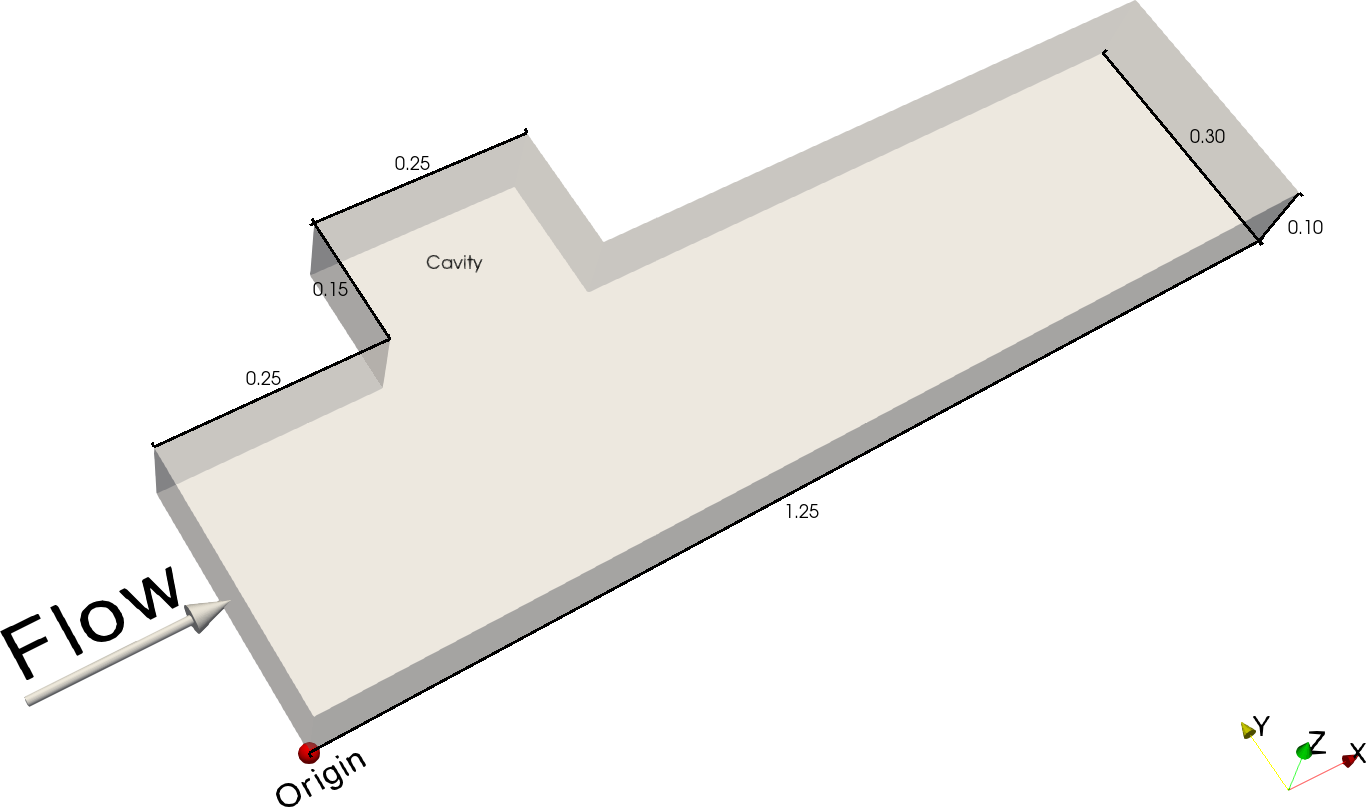
\includegraphics[width=\linewidth]{../images/art4/domain.png}
\caption{Computational domain with coordinates and dimensions.}
\label{fig:art4:domain}
\end{figure}

The boundary conditions set to the model were the following. The rigid-lid approximation was applied at the free surface of the domain ($z = 0.10$ m), which is valid for flows with $Fr < 0.5$ \cite{alfrink1983}. The longitudinal \textit{XZ} plane, located at $y=0$ m, where the main channel was restricted in the domain, was defined as a free-slip surface. Knowing that flow effects caused by obstacles to the main channel do not exceed one obstacle length \cite{Brevis2014}, and knowing that the cavity had $L=0.15$ m, we defined the width of the main channel to be $B=0.30$ m, which was sufficient to capture any flow effect in the main channel. The inlet portion of the domain ($x=0$ m) received precalculated velocity fields that were fully developed in a periodic channel, under the same flow conditions and the main channel geometry. The implementation of this boundary condition applied the turbulence Divergence-Free Synthetic Eddy Method (DF-SEM) to synthesise eddies based on the turbulence developed of the imported flow \cite{poletto2013}. A convective outflow boundary condition was adopted at the outlet ($x = 1.25$ m), in which the zero-gradient condition allows the flow to exit the domain without having any backflow. The bottom of the domain ($z = 0$ m) and the walls of the main channel ($y = 0.30$ m) and the cavity were considered as no-slip surfaces. 

The mass exchange between the main channel and the vegetated cavity was simulated with tracer fields, in which the washout procedure was implemented. After all the solution transients were eliminated, the lateral cavity was filled with an inert tracer. The flow was calculated until either all tracer left the cavity, or a time of 200 s passed. The associated turbulent Schmidt number was $S_{ct}=0.9$ , as used in other similar flows \cite{Gualtieri2017}. In this period, the average flow was, also, calculated and condensed into an ensemble averaging \cite{sukhodolov2014}. The computational time increment was held variable, with a Courant number kept under 0.90 and a maximum time step of 0.05 s.

The simulations were performed with the open-source package OpenFOAM (version 1912). To discretize the governing equations and numerical schemes, the module pimpleFoam, which employs the finite volume method (FVM), was used. For the pressure-velocity coupling, the PIMPLE method scheme was adopted. To solve the convection-diffusion equations, the implicit second-order backward time-stepping scheme and additional second-order schemes were used. The residual tolerance was set to $1 \times 10^{-4}$ and the number of our loops was set to 3, the same count was set for the pressure correction loops.

\subsection{Numerical Programme}
The study of the vegetated cavity was proposed by varying the vegetation density values using different DF coefficients to emulate the increasing drag, which is summarised in Table \ref{tab:art4:cases}. The density was varied between $a = 0$ (no vegetation) and $a = 10.656$\%, distributed in ten scenarios for simulation. The vegetation density found in natural conditions varies from $0.001<a<0.45$, and the effects of the turbulence dissipation remains predominant until  $a<0.1$ \cite{Nepf2012}, given that these values were based on a free open channel, we chose a smaller value of a that could comprehend all the turbulence dissipation spectrum as this is a key component of the hydrodynamics of dead waters. It was assumed that the vegetation was uniformly distributed in the cavity and that it spanned the cavity depth, similarly to emergent vegetation.

\begin{table}[]
\centering
\begin{tabular}{@{}lllllll@{}}
\toprule
\multirow{2}{*}{Case} & \multirow{2}{*}{a (\%)} & \multicolumn{2}{l}{Horizontal direction (x and y-axis)} & \multicolumn{3}{l}{Vertical direction (z-axis)} \\ \cmidrule(l){3-7} 
   &         & $d$ (1/m2)   & $f$ (1/m) & $dh$ (m) & $d$ (1/m2)  & $f$ (1/m) \\ \midrule
0  & 0       & 0.00       & 0.00    & 0.00   & 0.00      & 0.00    \\
1  & 0.1332  & 116.53     & 3.09    & 0.7624 & 0.000451  & 0.00608 \\
2  & 0.1665  & 182.25     & 3.87    & 0.8265 & 0.0006    & 0.00702 \\
3  & 0.3330  & 753.83     & 7.89    & 0.3902 & 0.0111    & 0.0303  \\
4  & 0.6660  & 3002.72    & 15.82   & 0.1846 & 0.198     & 0.19    \\
5  & 1.3320  & 12344.01   & 32.40   & 0.0836 & 3.98      & 0.58    \\
6  & 2.6640  & 51244.51   & 67.36   & 0.0360 & 88.96     & 2.81    \\
7  & 3.9960  & 120314.00  & 105.38  & 0.0210 & 613.12    & 7.52    \\
8  & 5.3280  & 223190.20  & 146.57  & 0.0139 & 2602.53   & 15.83   \\
9  & 7.9920  & 546724.99  & 239.43  & 0.0072 & 23702.83  & 49.85   \\
10 & 10.6560 & 1061150.94 & 348.58  & 0.0041 & 140829.09 & 126.99  \\ \bottomrule
\end{tabular}
\caption{Vegetation levels and the calculated Darcy-Forchheimer coefficients, where $a$ (\%) is the vegetation density, $d$ (1/m2) is the viscosity drag coefficient, $f$ (1/m) is the inertial coefficient and $dh$ (m) is the hydraulic diameter.}
\label{tab:art4:cases}
\end{table}
\subsection{LES Quality and Grid Independence}
The quality of the numerical solution was evaluated using a procedure based on three different grids \cite{Dutta2018}. The refinement rate between the grids was 1.80, although with the same configurations (numerical model and boundary conditions). The numerical and modelling errors were estimated and compared to the experimental data from \textcite{xiang2019}. Figure \ref{fig:art4:validation} shows the ensemble-averaged streamwise velocity with the total error (numerical and modelled) expressed by error bars. Overall, the numerical solution presented low error magnitudes, with a mean total error of –0.0024 m/s. The errors could be mitigated by a further refinement, although the errors were small enough to continue the experiments.

\begin{figure}[!ht]
\centering
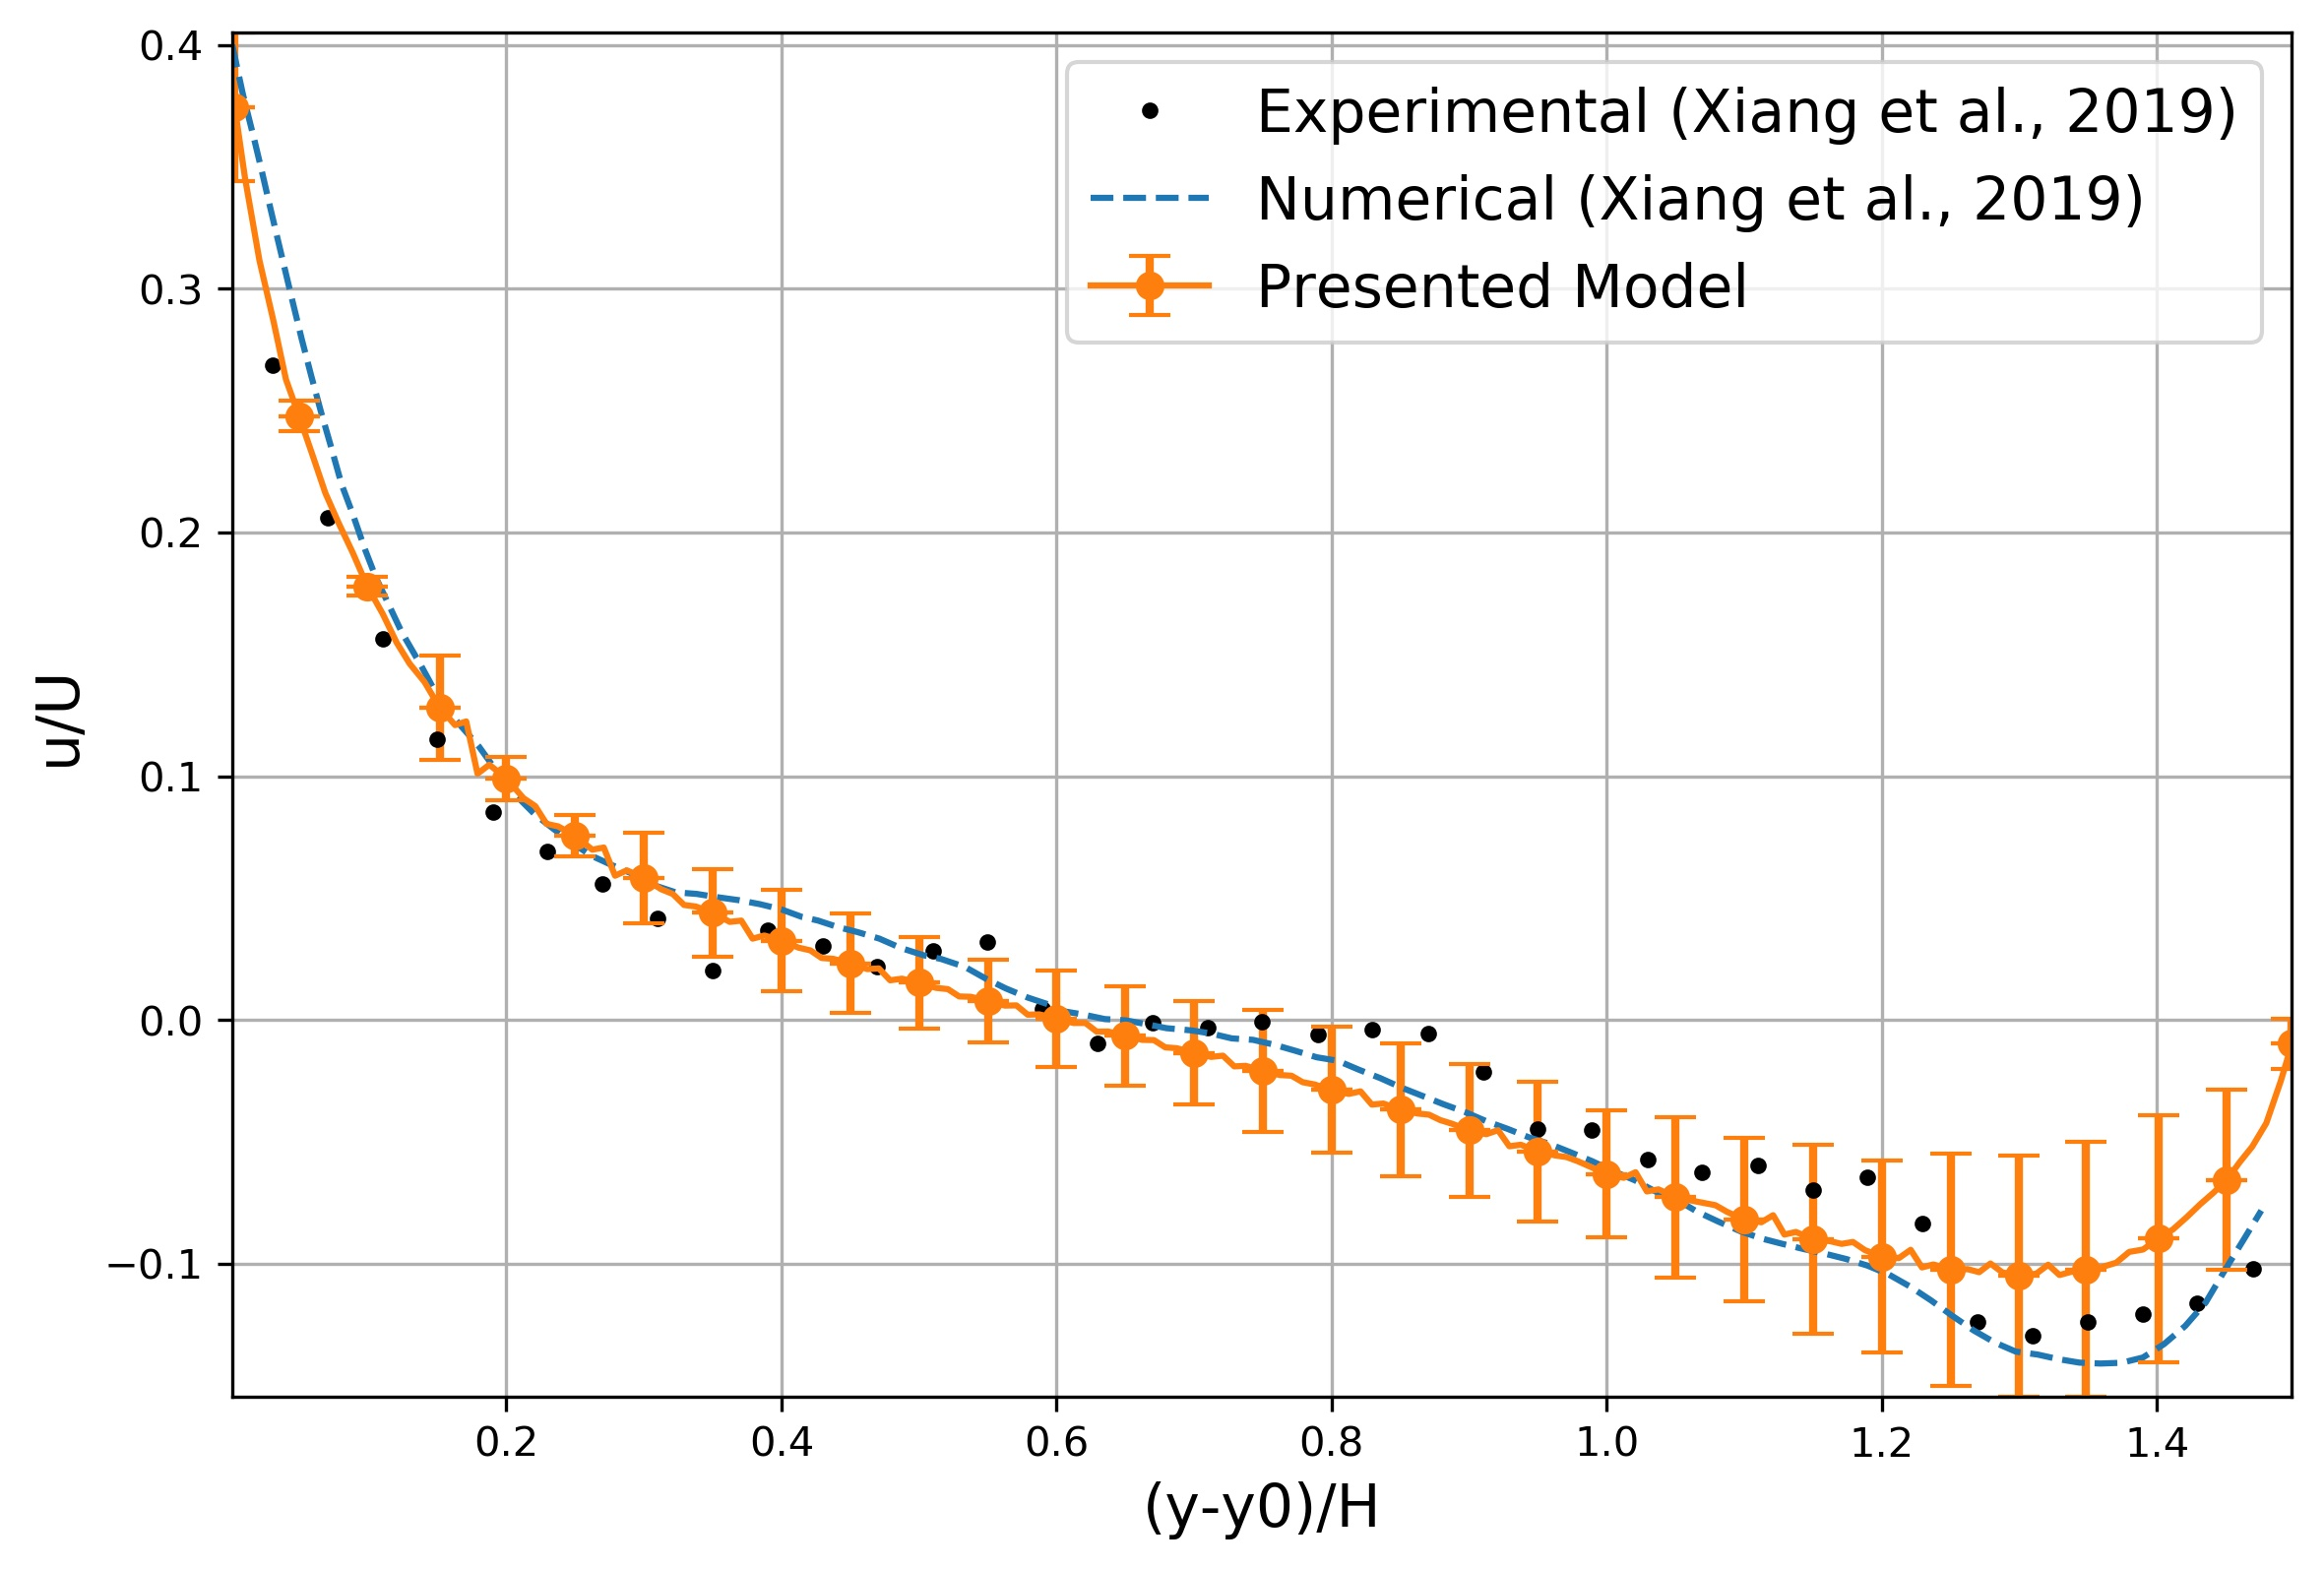
\includegraphics[width=\linewidth]{../images/art4/validation.jpeg}
\caption{Grid and Numerical Errors of the ensemble-averaged streamwise velocity in the cavity at $z=0.6H$, where $U$ is the bulk velocity in the main channel, $y_0=0.30$m represents the beginning of the cavity and $H$ is the height of the flow.}
\label{fig:art4:validation}
\end{figure}
\subsection{Validation}
Figure \ref{fig:art4:validation} compares the results of the time-averaged streamwise velocity \textit{u} at $z/H=0.6$ obtained from the second case ($a=0.1332$\%) of \textcite{xiang2019}, using both experimental and his numerical model. The numerical results, from the present paper, showed good consistency with the experimental data. A difference between the wall resolved LES (WRLES) and the wall modelled LES (WMLES) is highlighted in the region $(y-y_0)/H > 1.20$, where the continuous line deviated from the dashed result. Although, in all other regions the results followed closely both experimental and the WRLES.

\section{Flow Characteristics}
Figure \ref{fig:art4:velocityContour} show the mean 2D streamlines for all the cases at $z/H=0.6$. Under the cases 0 to 5 a main anti-clockwise motion takes place (Figure \ref{fig:art4:velocityContour}  a-f). The increase in vegetation density translates the centre of the gyre towards the main channel and downstream in the x-direction as the blockage effects increase and the flow loses energy faster. For $a=1.3320$\% (case 5) the main circulation starts to lose its shape and this process continues up to $a=3.9960$\% when the flow stabilised (Figure \ref{fig:art4:velocityContour}  f and Figure \ref{fig:art4:velocityContour}  g-h). The case 8 showed the formation of a secondary gyre system at the right portion of the cavity, $0.45<x/L<1$ and $0<y/W<1$ (Figure \ref{fig:art4:velocityContour}  i). This behaviour was shifted to the left as the vegetation increased to $a=7.9920$\% (Case 9), $0.30<x/L<1$ and $0<y/W<1$ (Figure \ref{fig:art4:velocityContour}  i). The presence of secondary circulations normally occurs at different aspect ratios: $W/L<0.5$ and $W/L>1.5$ \cite{Sukhodolov2002}, this circulation naturally does not have any contact with the main channel as they are derived from the primary circulation. Figure \ref{fig:art4:velocityContour}  i-k show the primary circulation at the bottom left of the cavity and the secondary gyre occupying approximately 50\% of the area in $a=5.3280$\%, the area comprehending the secondary gyre further increased with the vegetation drag increase.

Figure \ref{fig:art4:velXYPlane} show the flow at the horizontal plane \textit{XY} at $z/H = 0.6$ along the \textit{y}-axis, $(y-y_0)/H$ being $y_0=0.30$m the beginning of the cavity, where the velocity decreases as the vegetation density increases. Another important aspect of this figure is the positioning of the circulation centre that slowly shifts towards the region close to the interface ( $(y-y_0)/H=0$) that is associated with the flow resistance imposed by the vegetation.

\begin{figure}[!ht]
\centering
\includegraphics[width=\linewidth]{../images/art4/velocityContour.jpg}
\caption{Mean 2D streamlines of different vegetation densities at the horizontal plane $z/H = 0.6$: a) Case 0, b) Case 1, c) Case 2, d) Case 3, e) Case 4, f) Case 5, g) Case 6, h) Case 7, i) Case 8, j) Case 9 and k) Case 10.}
\label{fig:art4:velocityContour}
\end{figure}

\begin{figure}[!ht]
\centering
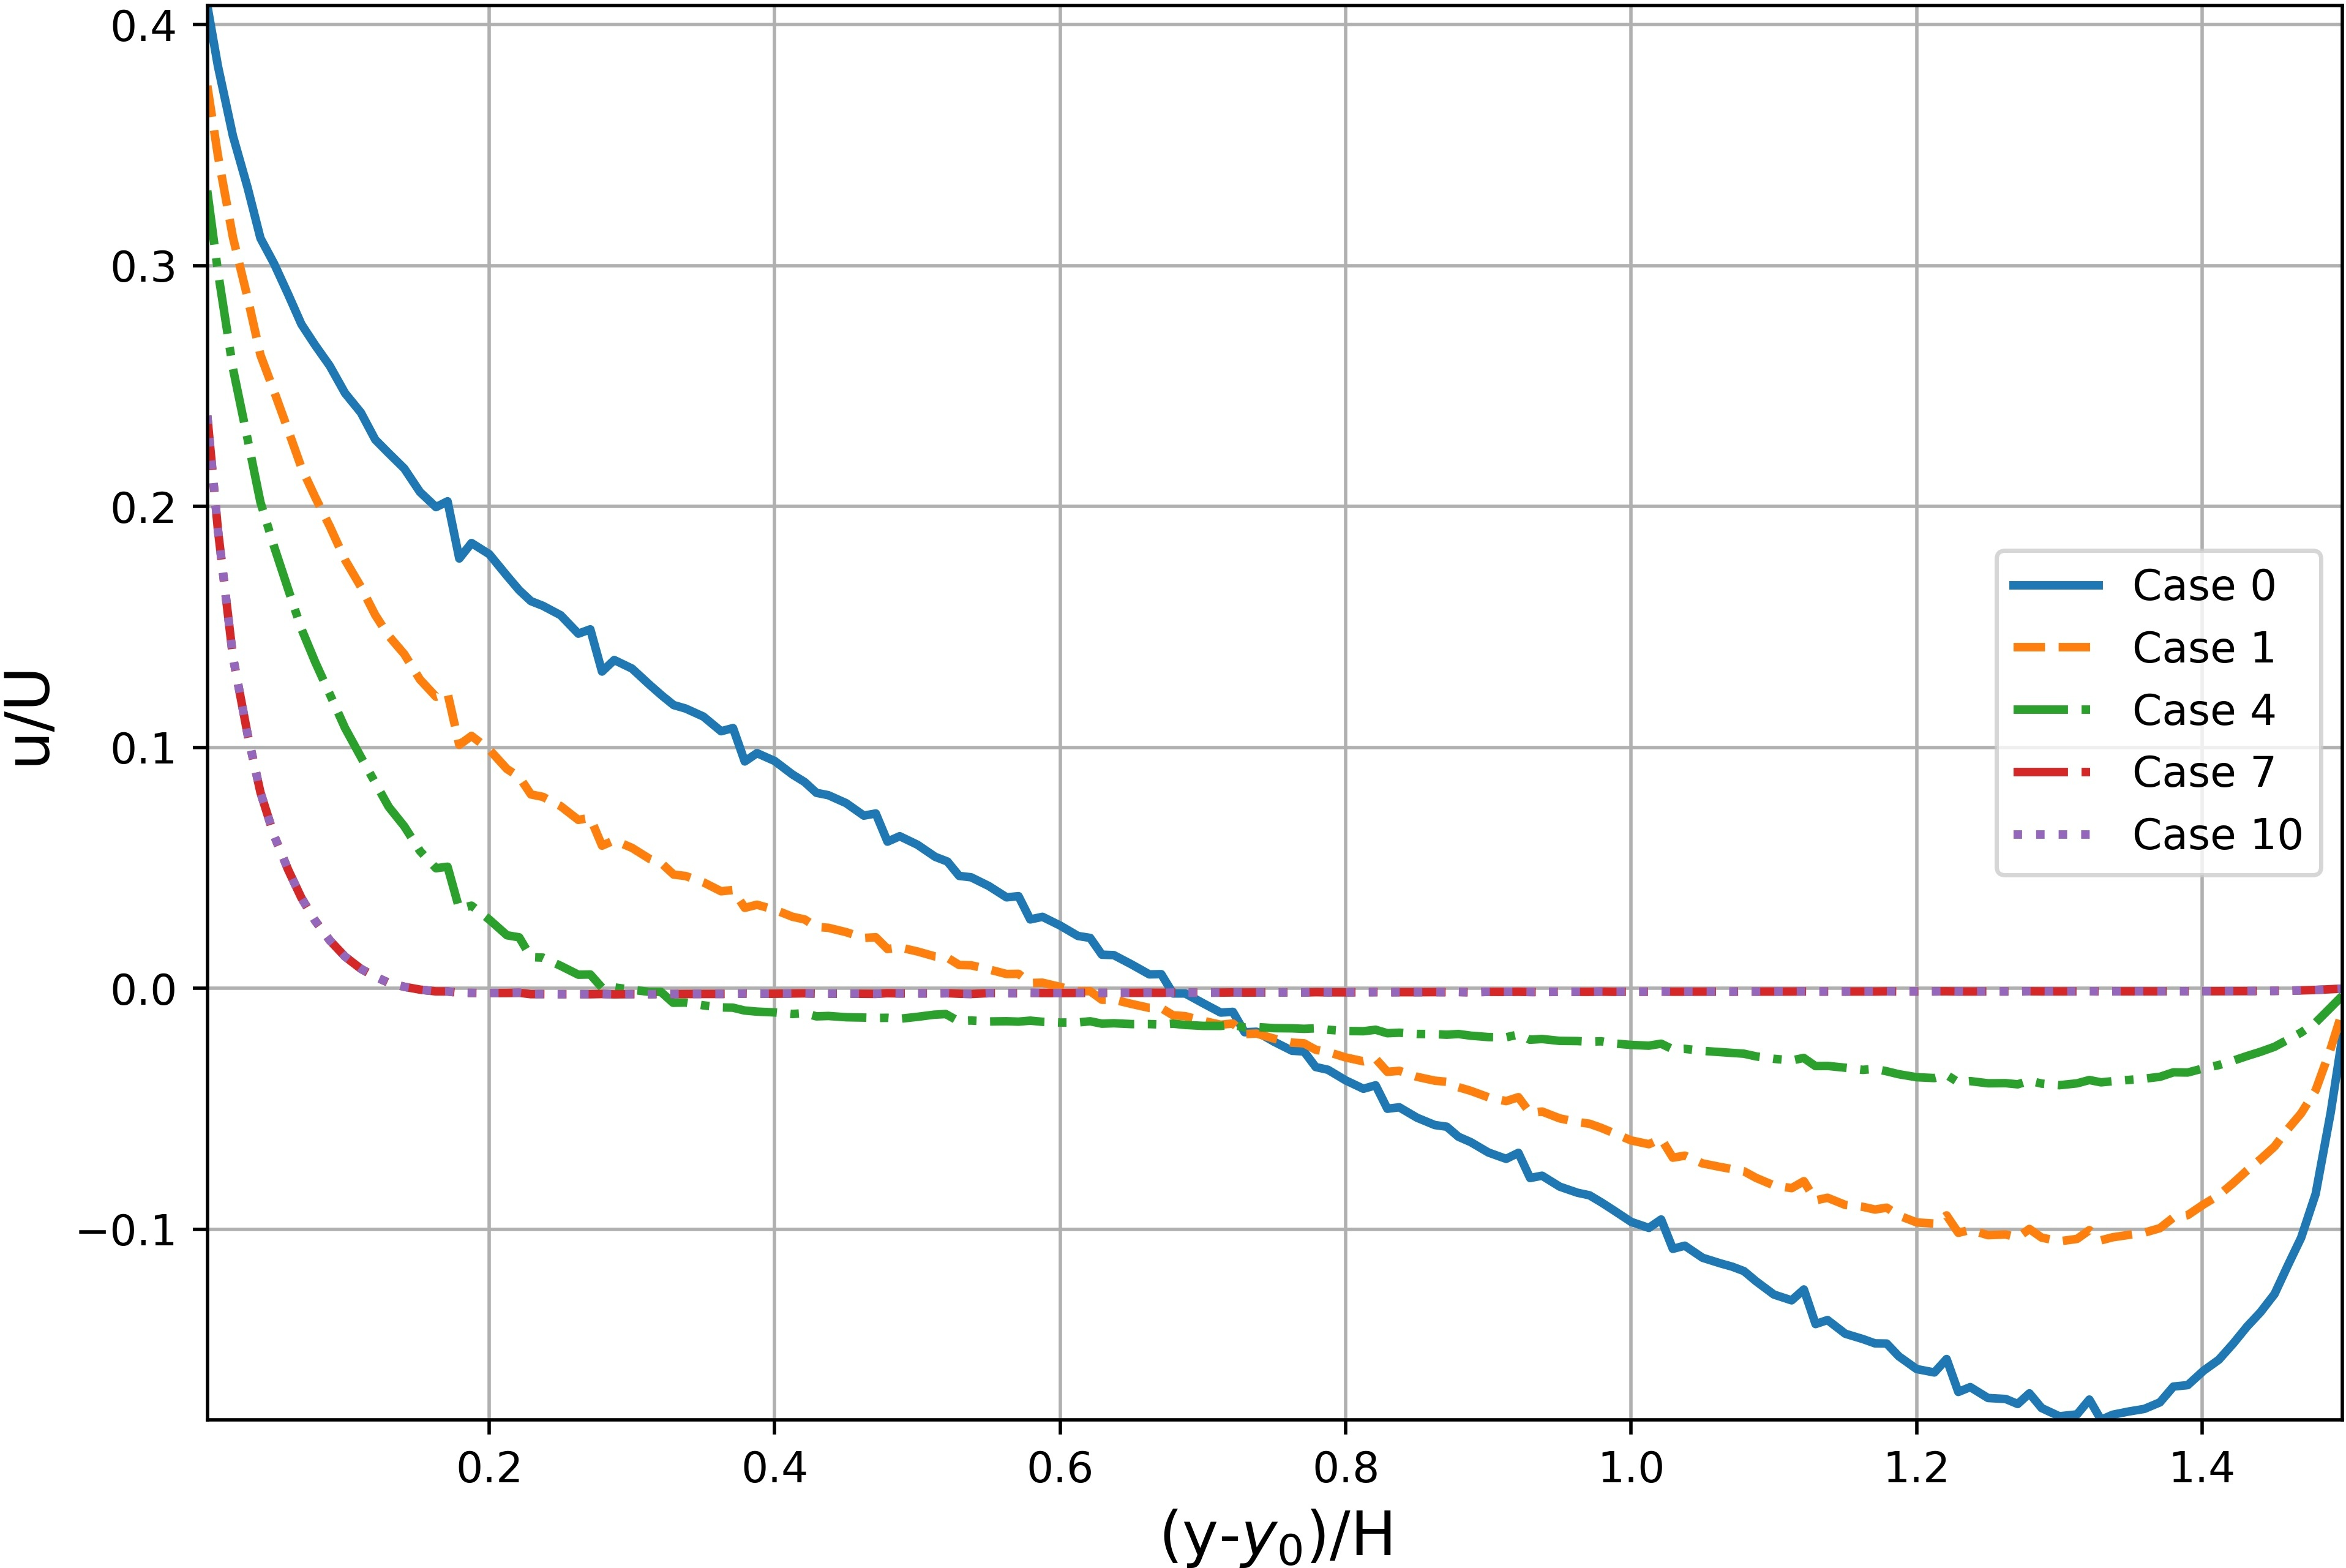
\includegraphics[width=\linewidth]{../images/art4/velXYPlane.jpg}
\caption{The variation of the streamwise velocity at the horizontal plane $z/H = 0.6$.}
\label{fig:art4:velXYPlane}
\end{figure}
The flow through the interface was initially directed toward the cavity ($z/H < 0.1$); positive velocity; then it was outwards ($0.1 < z/H < 0.9$); negative velocity; and lastly entering the domain ($z/H > 0.9$) (Figure \ref{fig:art4:yVelatInterfaceZAxis}). Through the variation in density, this behaviour did not change as the location of the phases did not change through all the cases, as seen in Figure \ref{fig:art4:yVelatInterfaceZAxis}, although the peak velocities at each phase gradually decreased as the vegetation density increased, which is attributable to the energy dissipation caused by vegetation. As the velocity values decreased the second phase ($0.1 < z/H < 0.9$) tended to flat as the vegetation was tending to a solid block behaviour similar to the behaviour of vegetation in \cite{chen2012}. Furthermore, the initial peak in velocity disappeared for $a > 5.32$\% (Case 8) and was substituted by the increase of the third phase.

\begin{figure}[!ht]
\centering
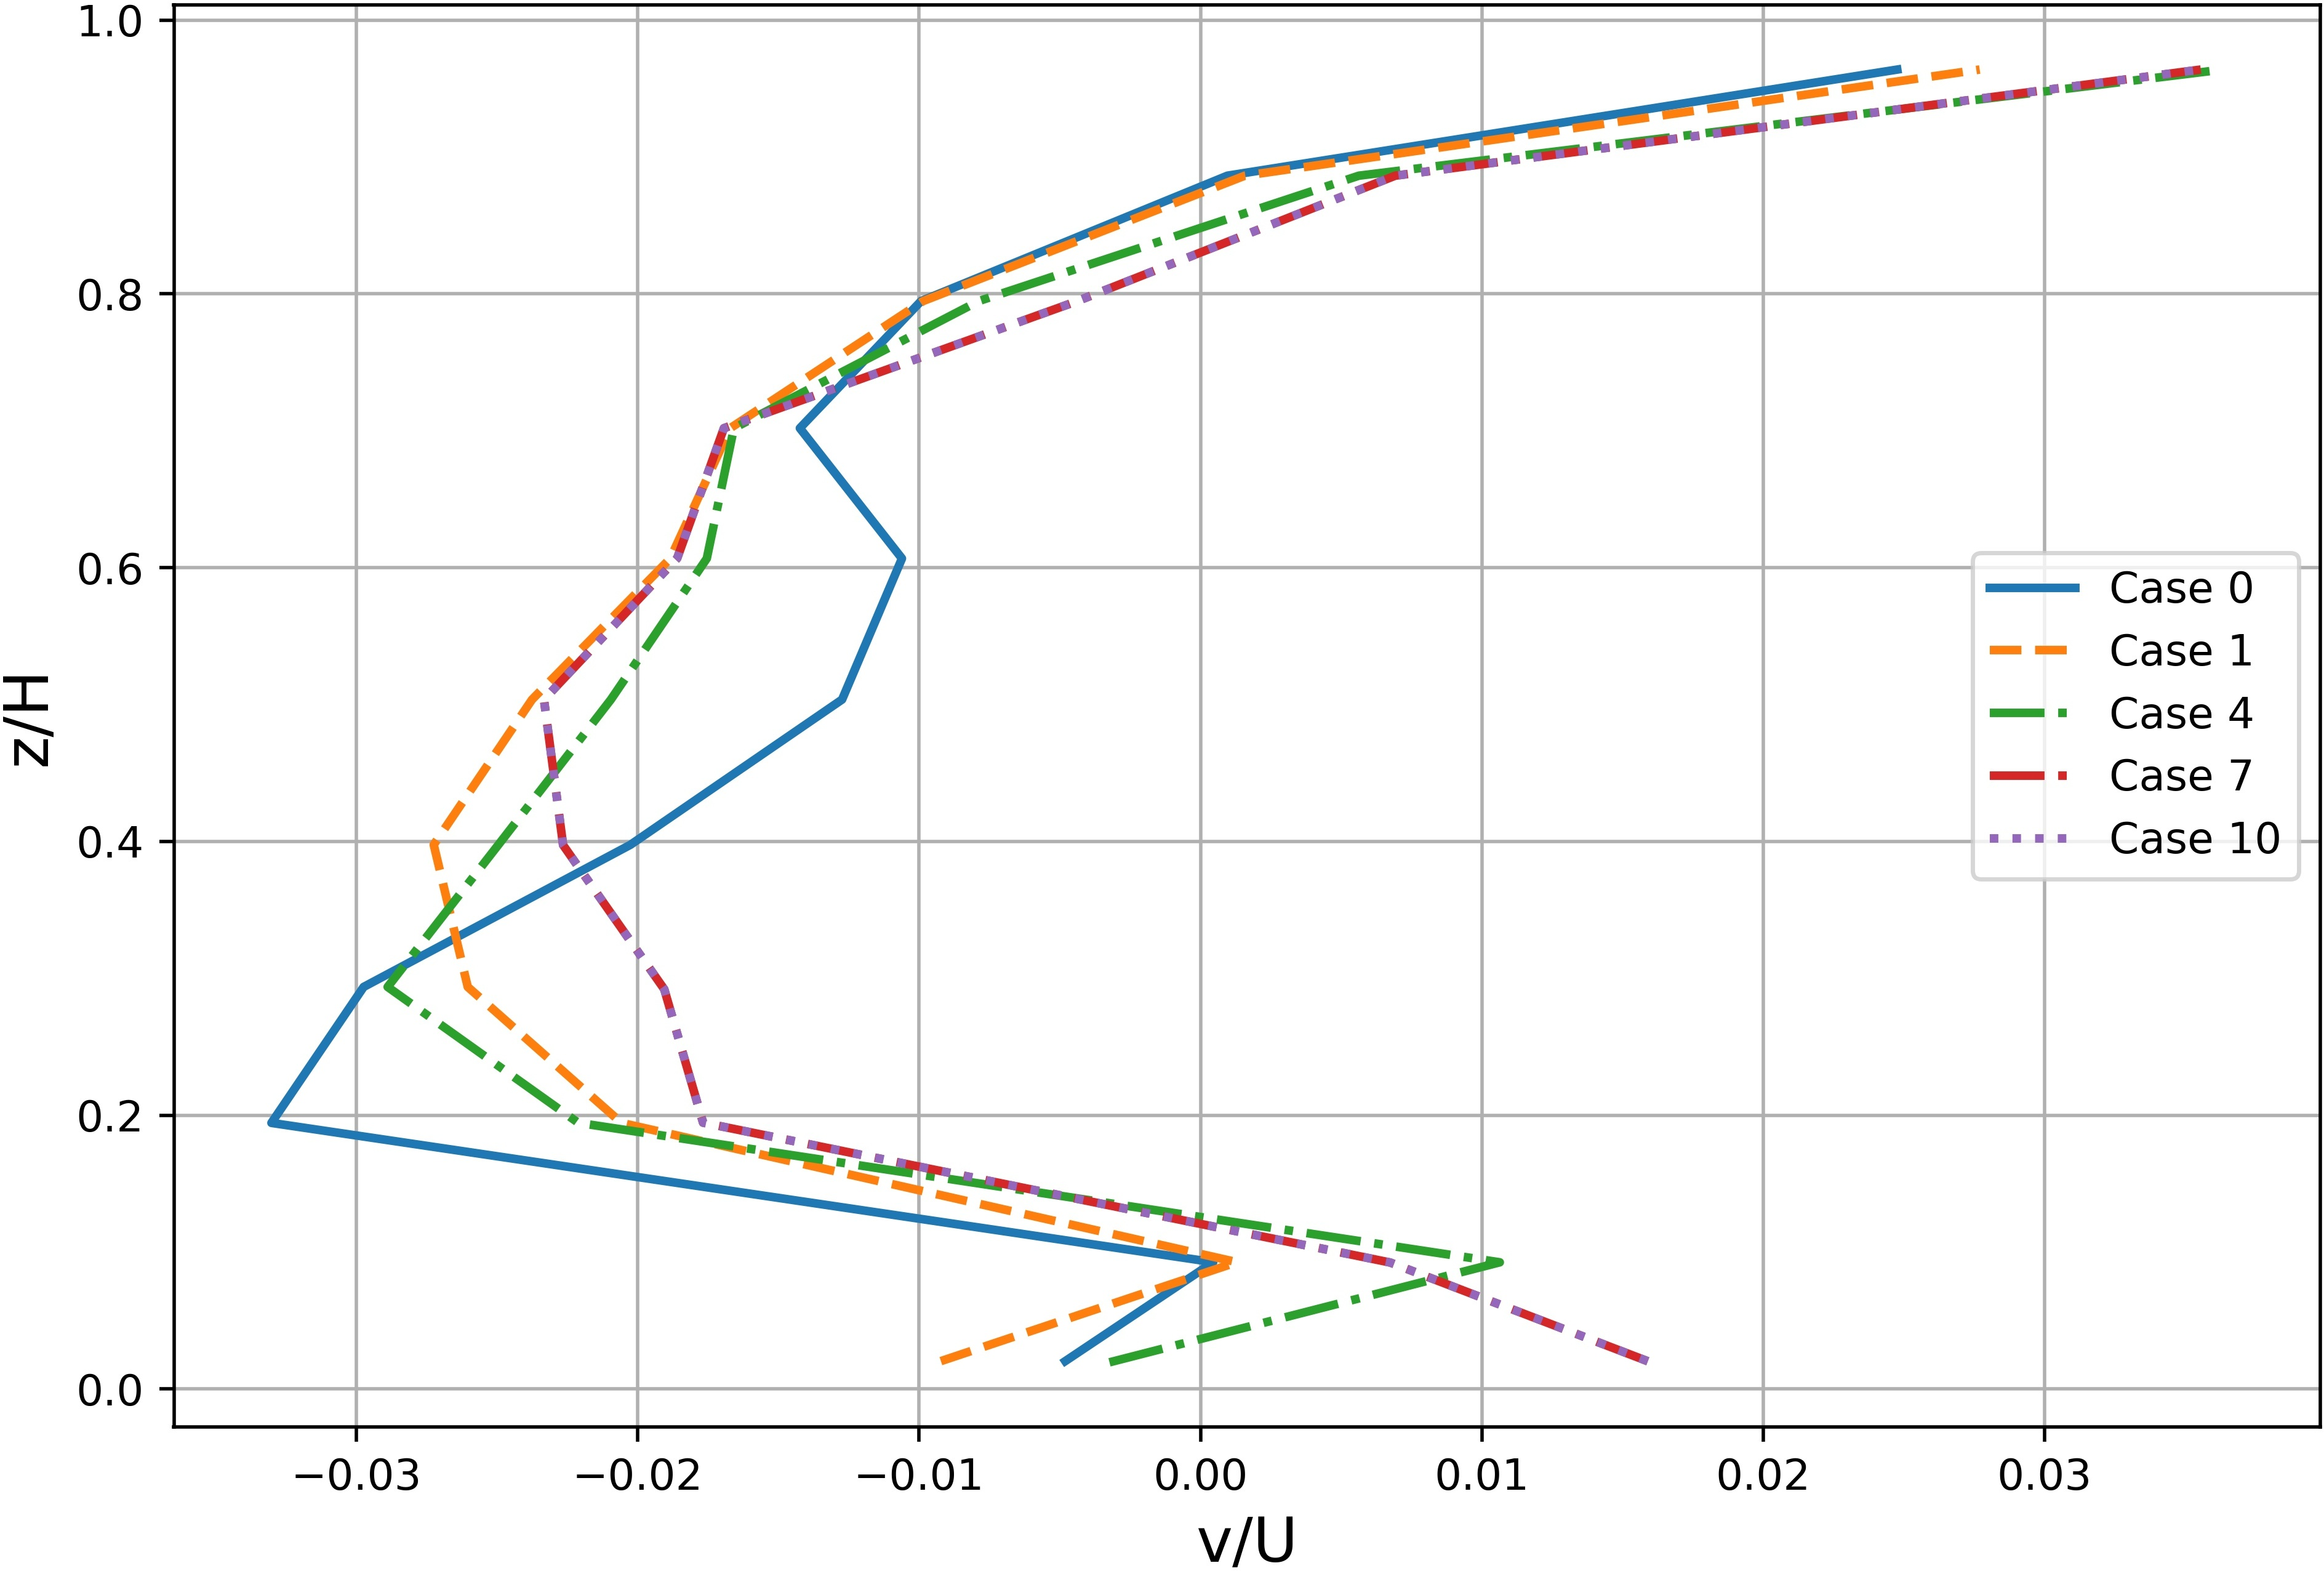
\includegraphics[width=\linewidth]{../images/art4/yVelatInterfaceZAxis.jpg}
\caption{The variation of the transversal velocity in the interface between the cavity and the main channel along the z-axis: a) Cases from 0 to 5; b) Cases from 5 to 10. Positive values of $v/U$ indicate the flow entering the cavity volume.}
\label{fig:art4:yVelatInterfaceZAxis}
\end{figure}

Figure \ref{fig:art4:yVelatInterfaceXAxis} shows the behaviour of the interface along the \textit{x}-axis. Analogous to the \textit{z}-axis, the increase in vegetation density altered the velocity zones. When the vegetation was not present, Case 0, the profile initially was set to the main channel up to 50 \% of the interface length similar to the behaviour of the series of groynes in \textcite{weitbrecht2004}. Although, with the increase of vegetation this first negative zone became positive and the only region where water exited the DZ volume was tending to $(x-x0)/L > 0.8$, due to the shock of the vortices to the downstream wall of the cavity.

\begin{figure}[!ht]
\centering
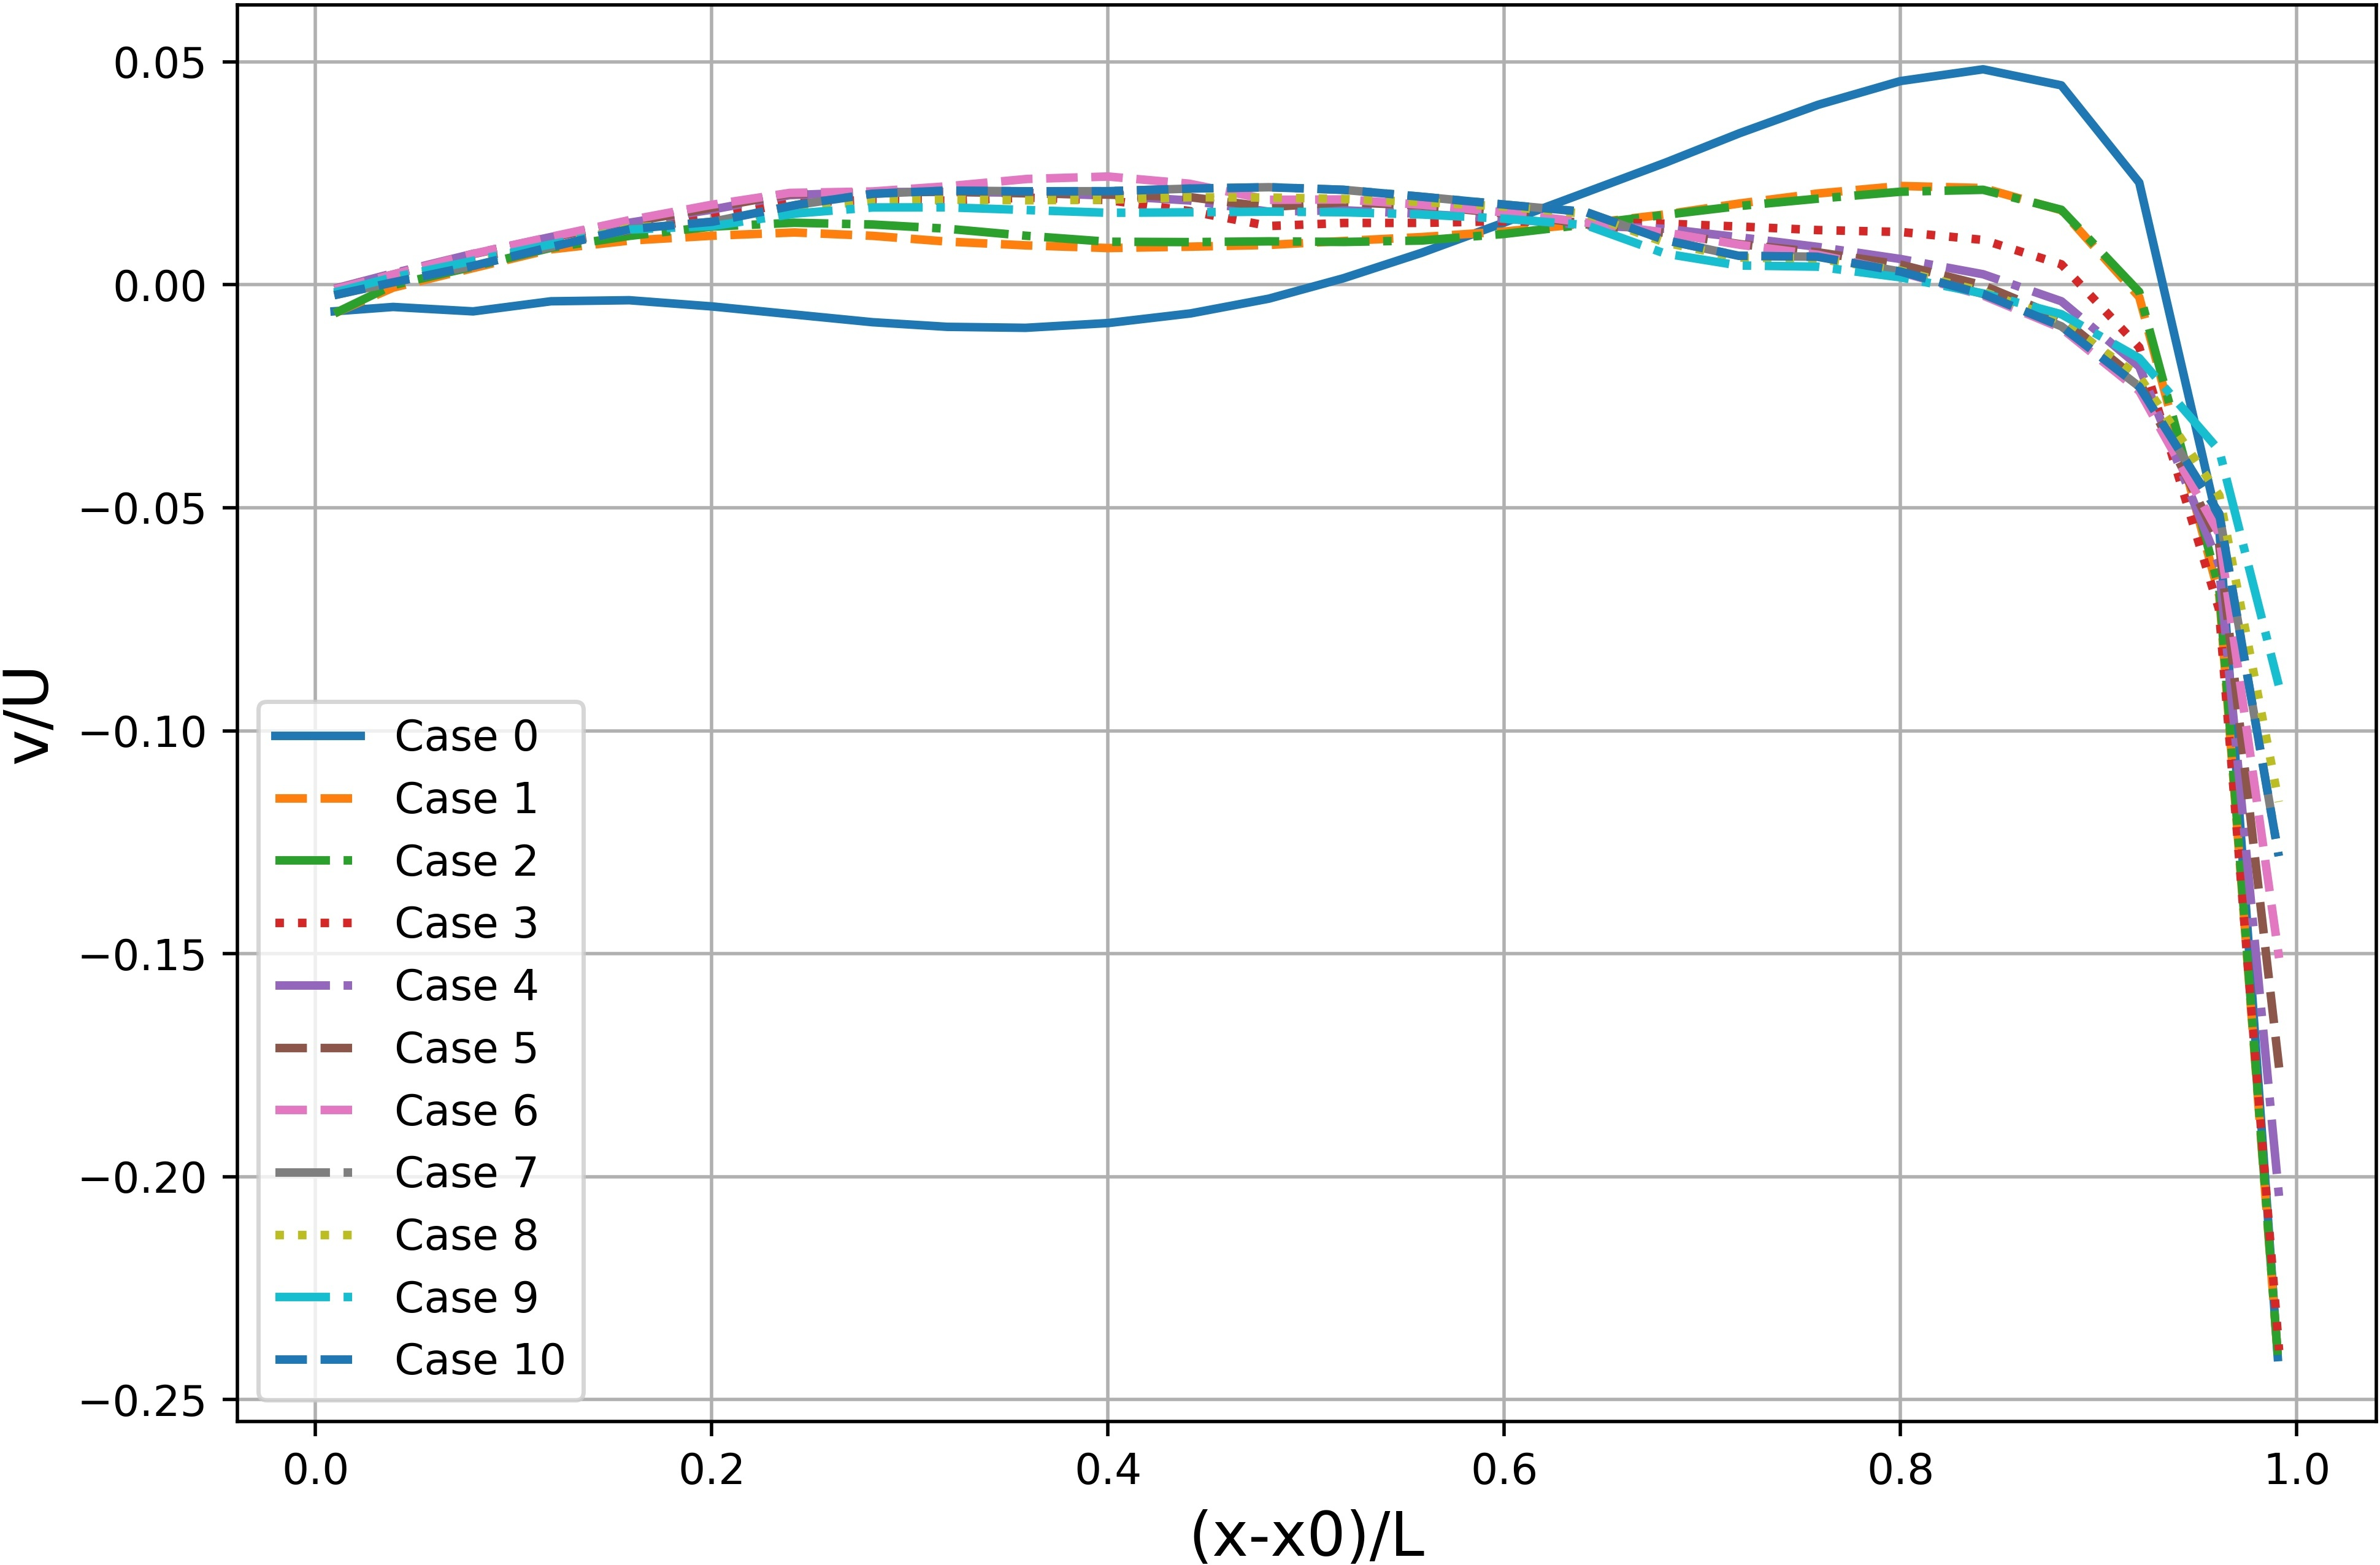
\includegraphics[width=\linewidth]{../images/art4/yVelatInterfaceXAxis.jpg}
\caption{The variation of the transversal velocity in the interface between the cavity and the main channel along the x-axis. Positive values of $v/U$ indicate the flow entering the cavity volume.}
\label{fig:art4:yVelatInterfaceXAxis}
\end{figure}

\section{Hydrodynamics of the Mixing Layer}
\subsection{Thickness of the Mixing Layer}
The mixing layer is a region that is developed along the interface due to a velocity gap between the lateral cavity and the main channel. The adoption of a thickness $\delta$  (m) of the mixing layer is commonly used to describe the spreading angle of the mixing layer and the range of velocity gradients between the zones \cite{xiang2020,Mignot2017,Yossef2011}. \textcite{xiang2020} suggested that the thickness could be divided into an inner section $\delta_{in}$  (m) (in the cavity) and an outer section $\delta_{out}$  (m) (in the main channel). The total thickness  is defined as:
\begin{equation}
\delta=\delta_{in}+\delta_{out}=\frac{U_i(x)-U_c(x)}{\left (\partial \bar{u} / \partial y  \right )_{max}}+\frac{U_m(x)+U_i(x)}{\left (\partial \bar{u} / \partial y  \right )_{max}}
\label{eqn:art4:thickness}
\end{equation}

where, $U_i$, $U_c$ and $U_m$ (m/s) are the time-averaged streamwise velocities at the interface, in the cavity and the main channel. These velocities were extracted where the velocity gradient is negligibly small, i.e., lower than 0.5 $s^{-1}$ in reference to \textcite{xiang2020,Mignot2017}. $\left (\partial \bar{u} / \partial y  \right )_{max}$ represents the maximum velocity gradient at each x position along the interface.

Figure \ref{fig:art4:thickness} show the evolution of the thickness layer in the streamwise direction for all the cases. Overall, the mixing layer increased when $(x-x_0)/L<0.80$ and decreased when $(x-x_0)/L>0.80$ as the velocity gradient increased in the contact with the wall. Similar to \textcite{xiang2020}, the vegetation density increase affected the width of the mixing layer, for both inner and outer sections. The increasing blockage limited the entrance of flow in the cavity (Figures \ref{fig:art4:velocityContour} and \ref{fig:art4:velXYPlane}), thus it limits the growth of the mixing layer. The wall behaviour of the cavity started to take place in case 8 and 9, although the presence of the secondary gyre in case 10 increased the thickness.

\begin{figure}[!ht]
\centering
\includegraphics[width=\linewidth]{../images/art4/thickness.jpeg}
\caption{Evolution of the mixing layer thickness averaged at the z-axis: a) inner mixing layer; b) outer mixing layer and c) total mixing layer.}
\label{fig:art4:thickness}
\end{figure}

\subsection{Vorticity}
Figures \ref{fig:art4:vorticityMean1} and \ref{fig:art4:vorticityMean2} show the time-averaged vorticity magnitude (normalised by U/H) at . The vorticity magnitude $\Omega$ ($s^{-1}$) is defined as:

\begin{equation}
\Omega = \nabla \times \vec{v}
\label{eqn:art4:vorticity}
\end{equation}

where, $\vec{v}$ (m/s) is the velocity vector.

For all cases, the vorticity remained high through all the interface between the cavity and the main channel. The maximum vorticity occurred at the upstream of the interface ($x/L<0.3$) and decreases in the downstream direction ($x/L>0.3$). Similar to groynes, this effect occurs to the shredding of vortex from the beginning of the cavity \textcite{xiang2020}. As the eddies shred, the high vorticity region increases in width (\textit{y}-axis) to its maximum value at the downstream wall. This width reduces as the vegetation density increases due to higher drag.

The increase of vegetation density gradually decreased the levels of vorticity inside the cavity volume up to $a<7.9920$, when there was no more vorticity in the volume. Although, it seems that vegetation increased the vorticity at the inner part of the mixing layer despite the blockage effect.

\begin{figure}[!ht]
\centering
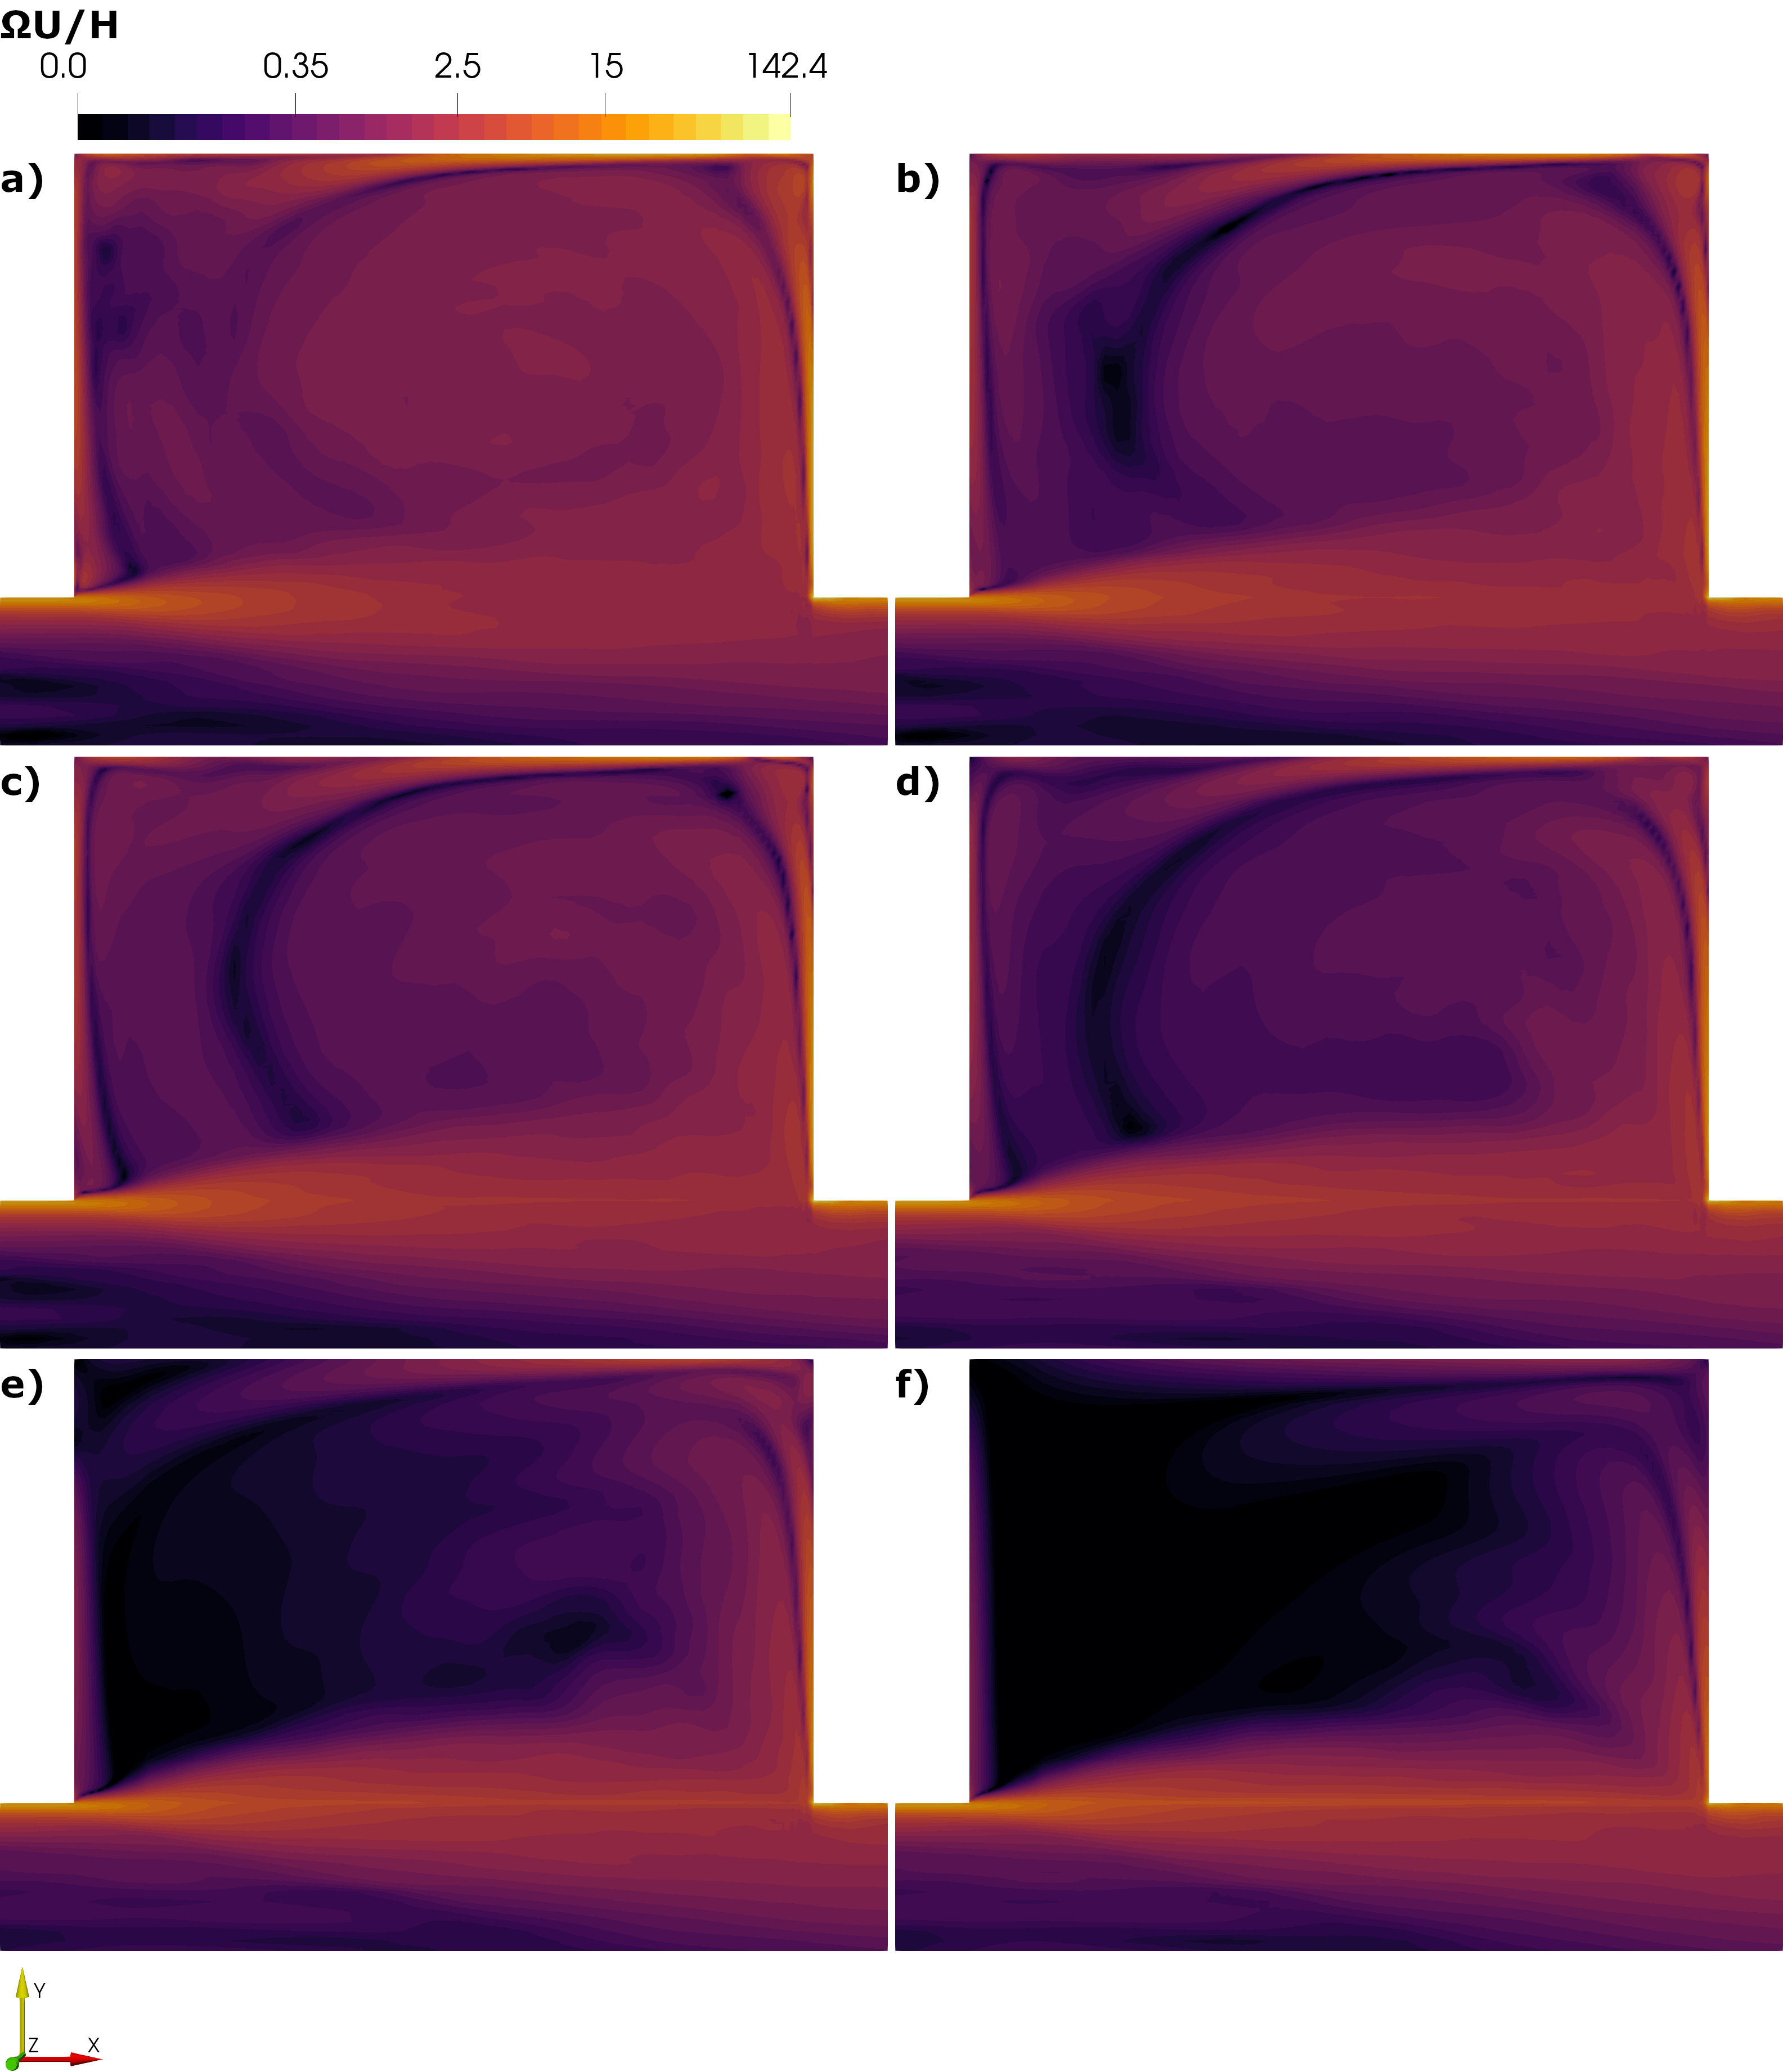
\includegraphics[width=\linewidth]{../images/art4/vorticityMean1.jpeg}
\caption{Time averaged vorticity at z/H = 0.6: a) Case 0, b) Case 1, c) Case 2, d) Case 3, e) Case 4 and f) Case 5.}
\label{fig:art4:vorticityMean1}
\end{figure}

\begin{figure}[!ht]
\centering
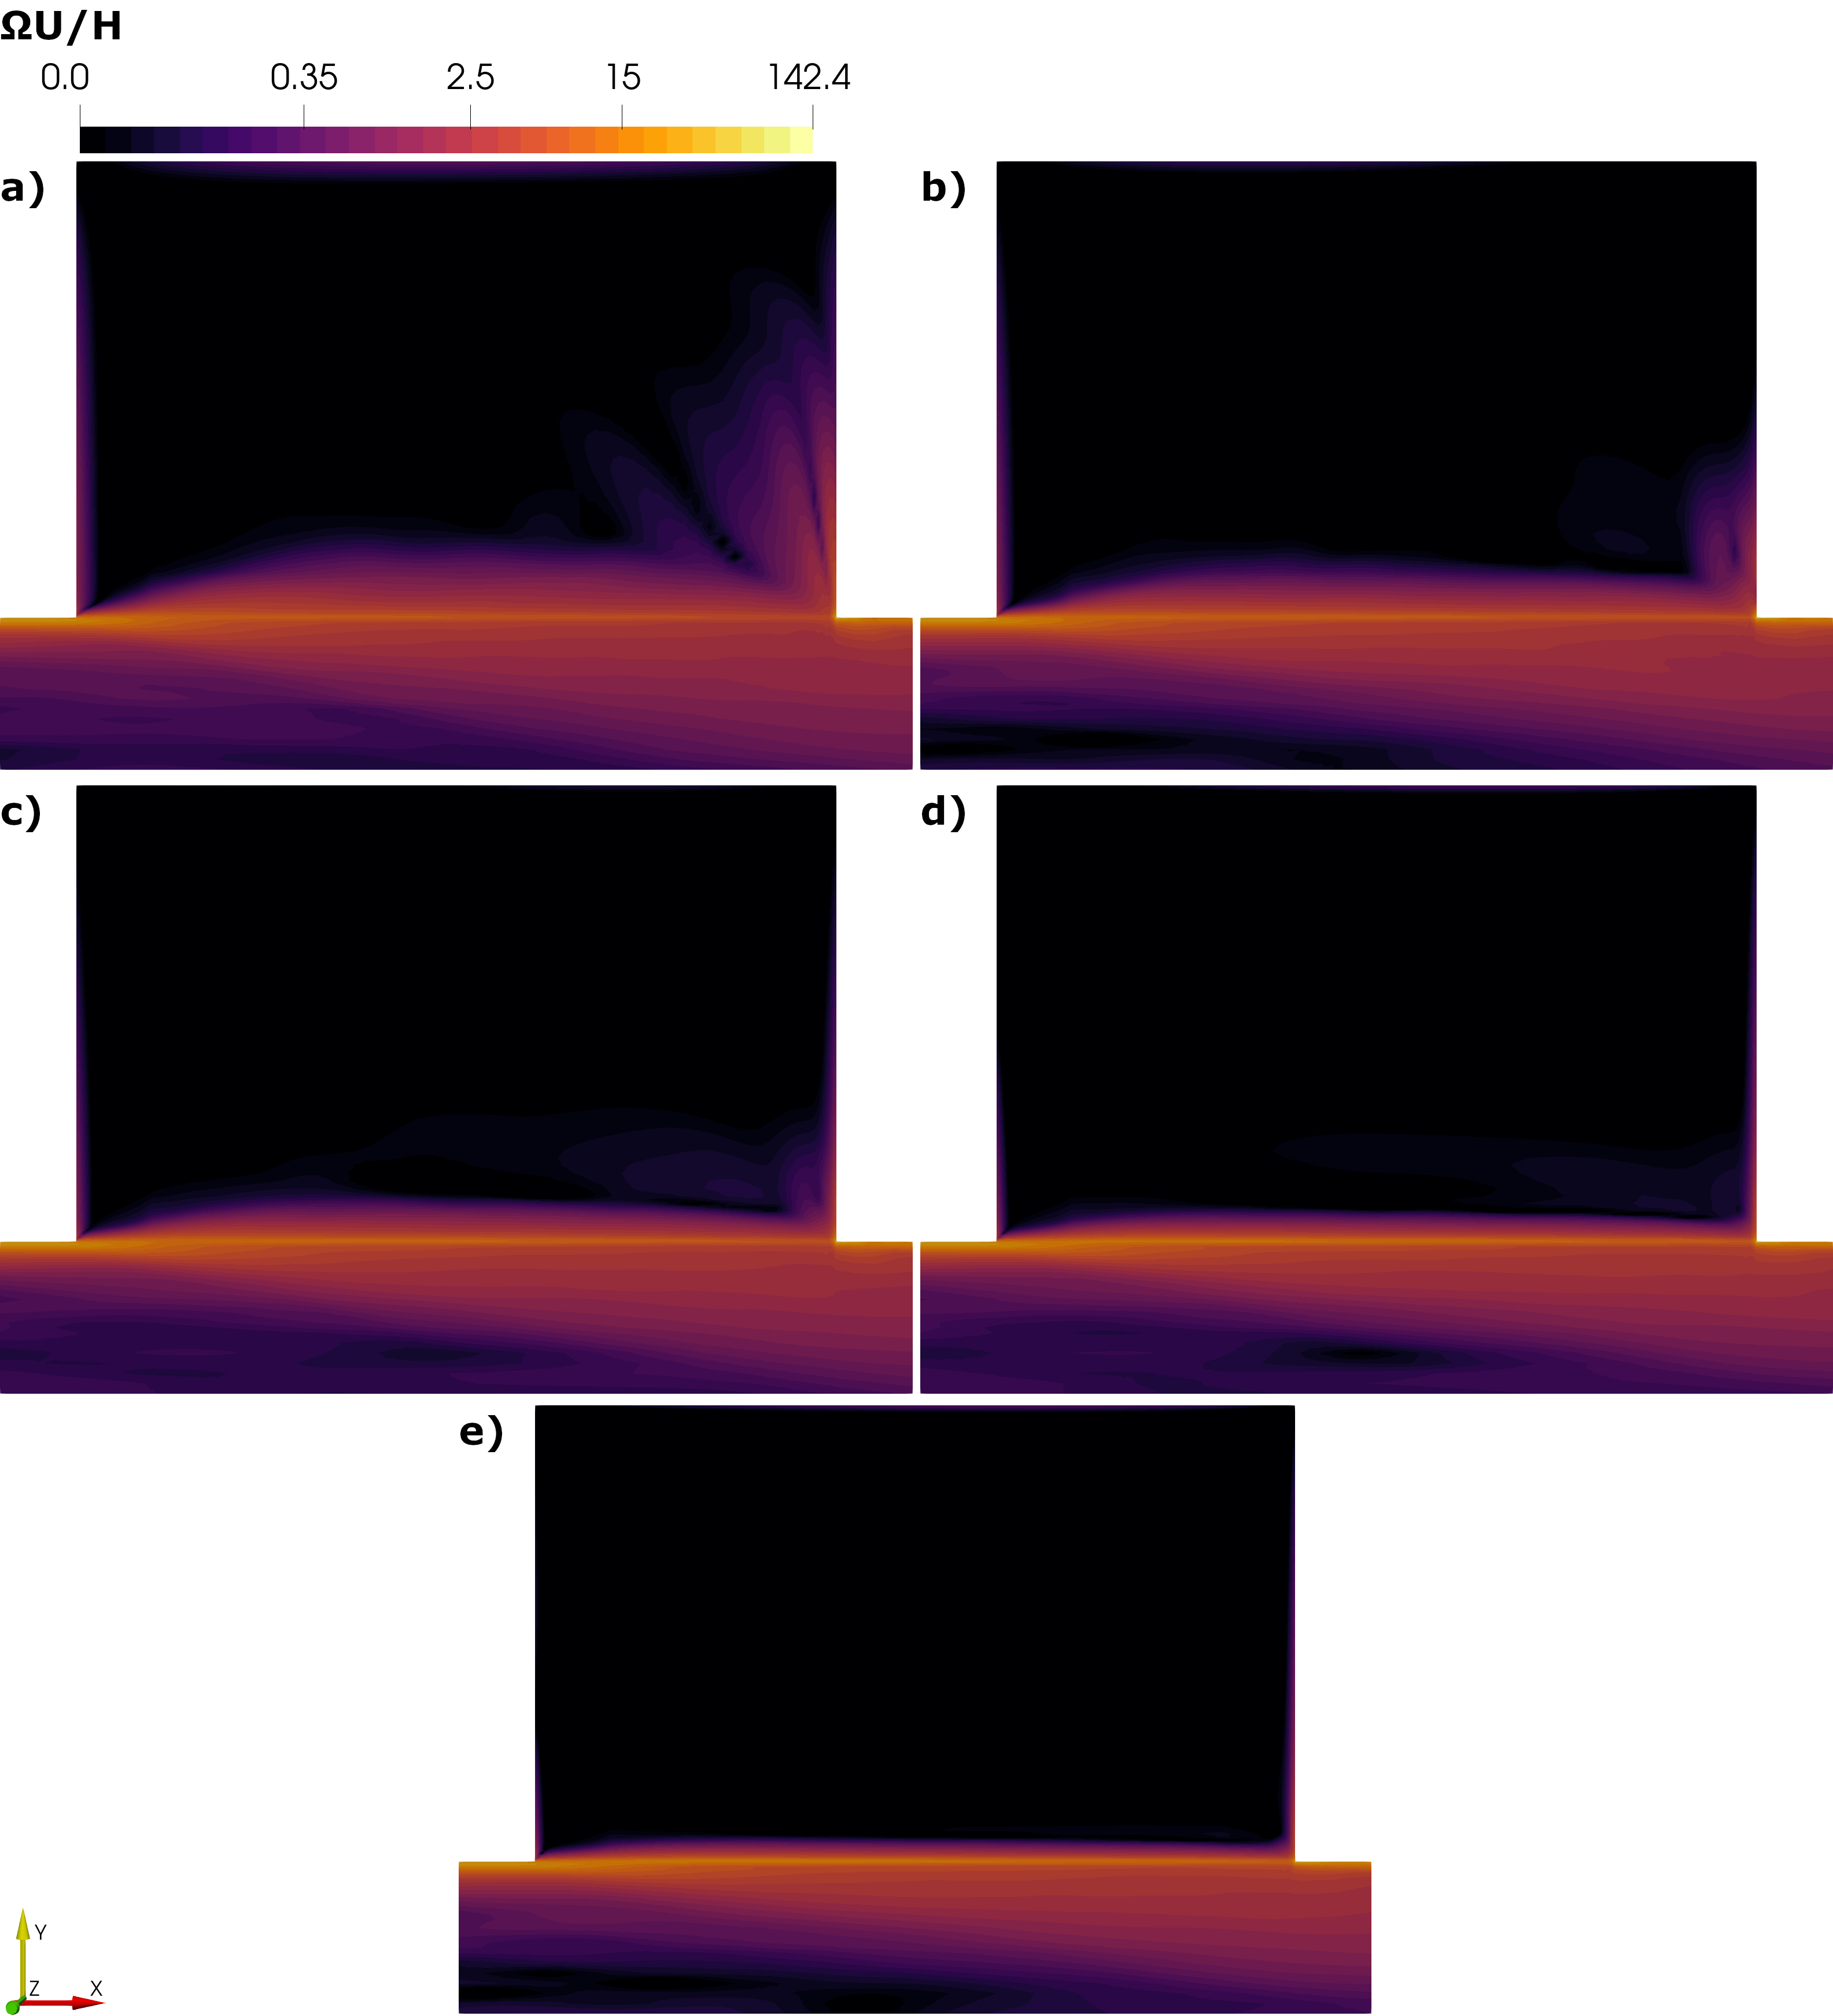
\includegraphics[width=\linewidth]{../images/art4/vorticityMean2.jpeg}
\caption{Time averaged vorticity at z/H = 0.6: a) Case 6, b) Case 7, c) Case 8, d) Case 9 and e) Case 10.}
\label{fig:art4:vorticityMean2}
\end{figure}

\subsection{Turbulent Kinetic Energy (TKE)}
The turbulent kinetic energy (TKE) in a LES simulation is defined as:
\begin{equation}
TKE = 0.5 tr(R) + 0.5 tr(u')
\label{eqn:art4:tke}
\end{equation}

where, $R$ (m2/s2) is the Reynolds stress tensor and $u’$ (m/s) is the instantaneous fluctuation tensor.

A time-averaged TKE distribution, normalised by $U^2$, is presented in Figures \ref{fig:art4:totalTKEMean1} and \ref{fig:art4:totalTKEMean2}. Through all interface, the values of TKE remained above $TKE/U^2 > 0.05$, at the downstream of the interface the maximum value occurred. At this same region, the vortex encounters the cavity lateral wall, the portion that enters the cavity reduces in magnitude as it moves through the vegetation. In an unvegetated scenario Figure \ref{fig:art4:totalTKEMean1} a) the TKE followed all the main circulation, behaviour that did not occur with the presence of vegetation. Hence the increase in vegetation density reduced the values of TKE, analogously to the vorticity.

As the vegetation density increased, the turbulent kinetic energy inside the cavity decreased, similarly to \textcite{xiang2019}, although in a much faster rate than the vorticity. The blockage effect due to the vegetation density increase slowly reduces the TKE values inside the cavity. The last region in which $TKE > 0$ is the downstream wall of the cavity, region where the first jet enters the volume. Similar to \textcite{xiang2019}, the first levels of vegetation registered an increase of TKE at the interface. Although with the increase of vegetation beyond $a > 0.33$\% (Figure \ref{fig:art4:totalTKEMean1} d), the turbulence intensity was lower than the non vegetated scenario which can be attributed to the shrink of the inner part of the mixing layer (Figure \ref{fig:art4:thickness} a) caused by the flow turbulence inhibition caused by high-density vegetation \cite{Nepf2012}. Furthermore, the shape of the TKE distribution on the outer part of the mixing layer changed with the increase of vegetation, on $a = 0$\% the region that the distribution width increases is up to approximately $(x-x0)/L < 0.8$, when the jet entrance to the volume decreases its width. For the vegetated cases, specially Case 3, the vegetation blocks part of the jet that normally enters the downstream portion of the volume, this causes the TKE distribution to take a triangular shape which indicates an increased turbulence intensity in the main channel up to $a < 5.328$ \%.

\begin{figure}[!ht]
\centering
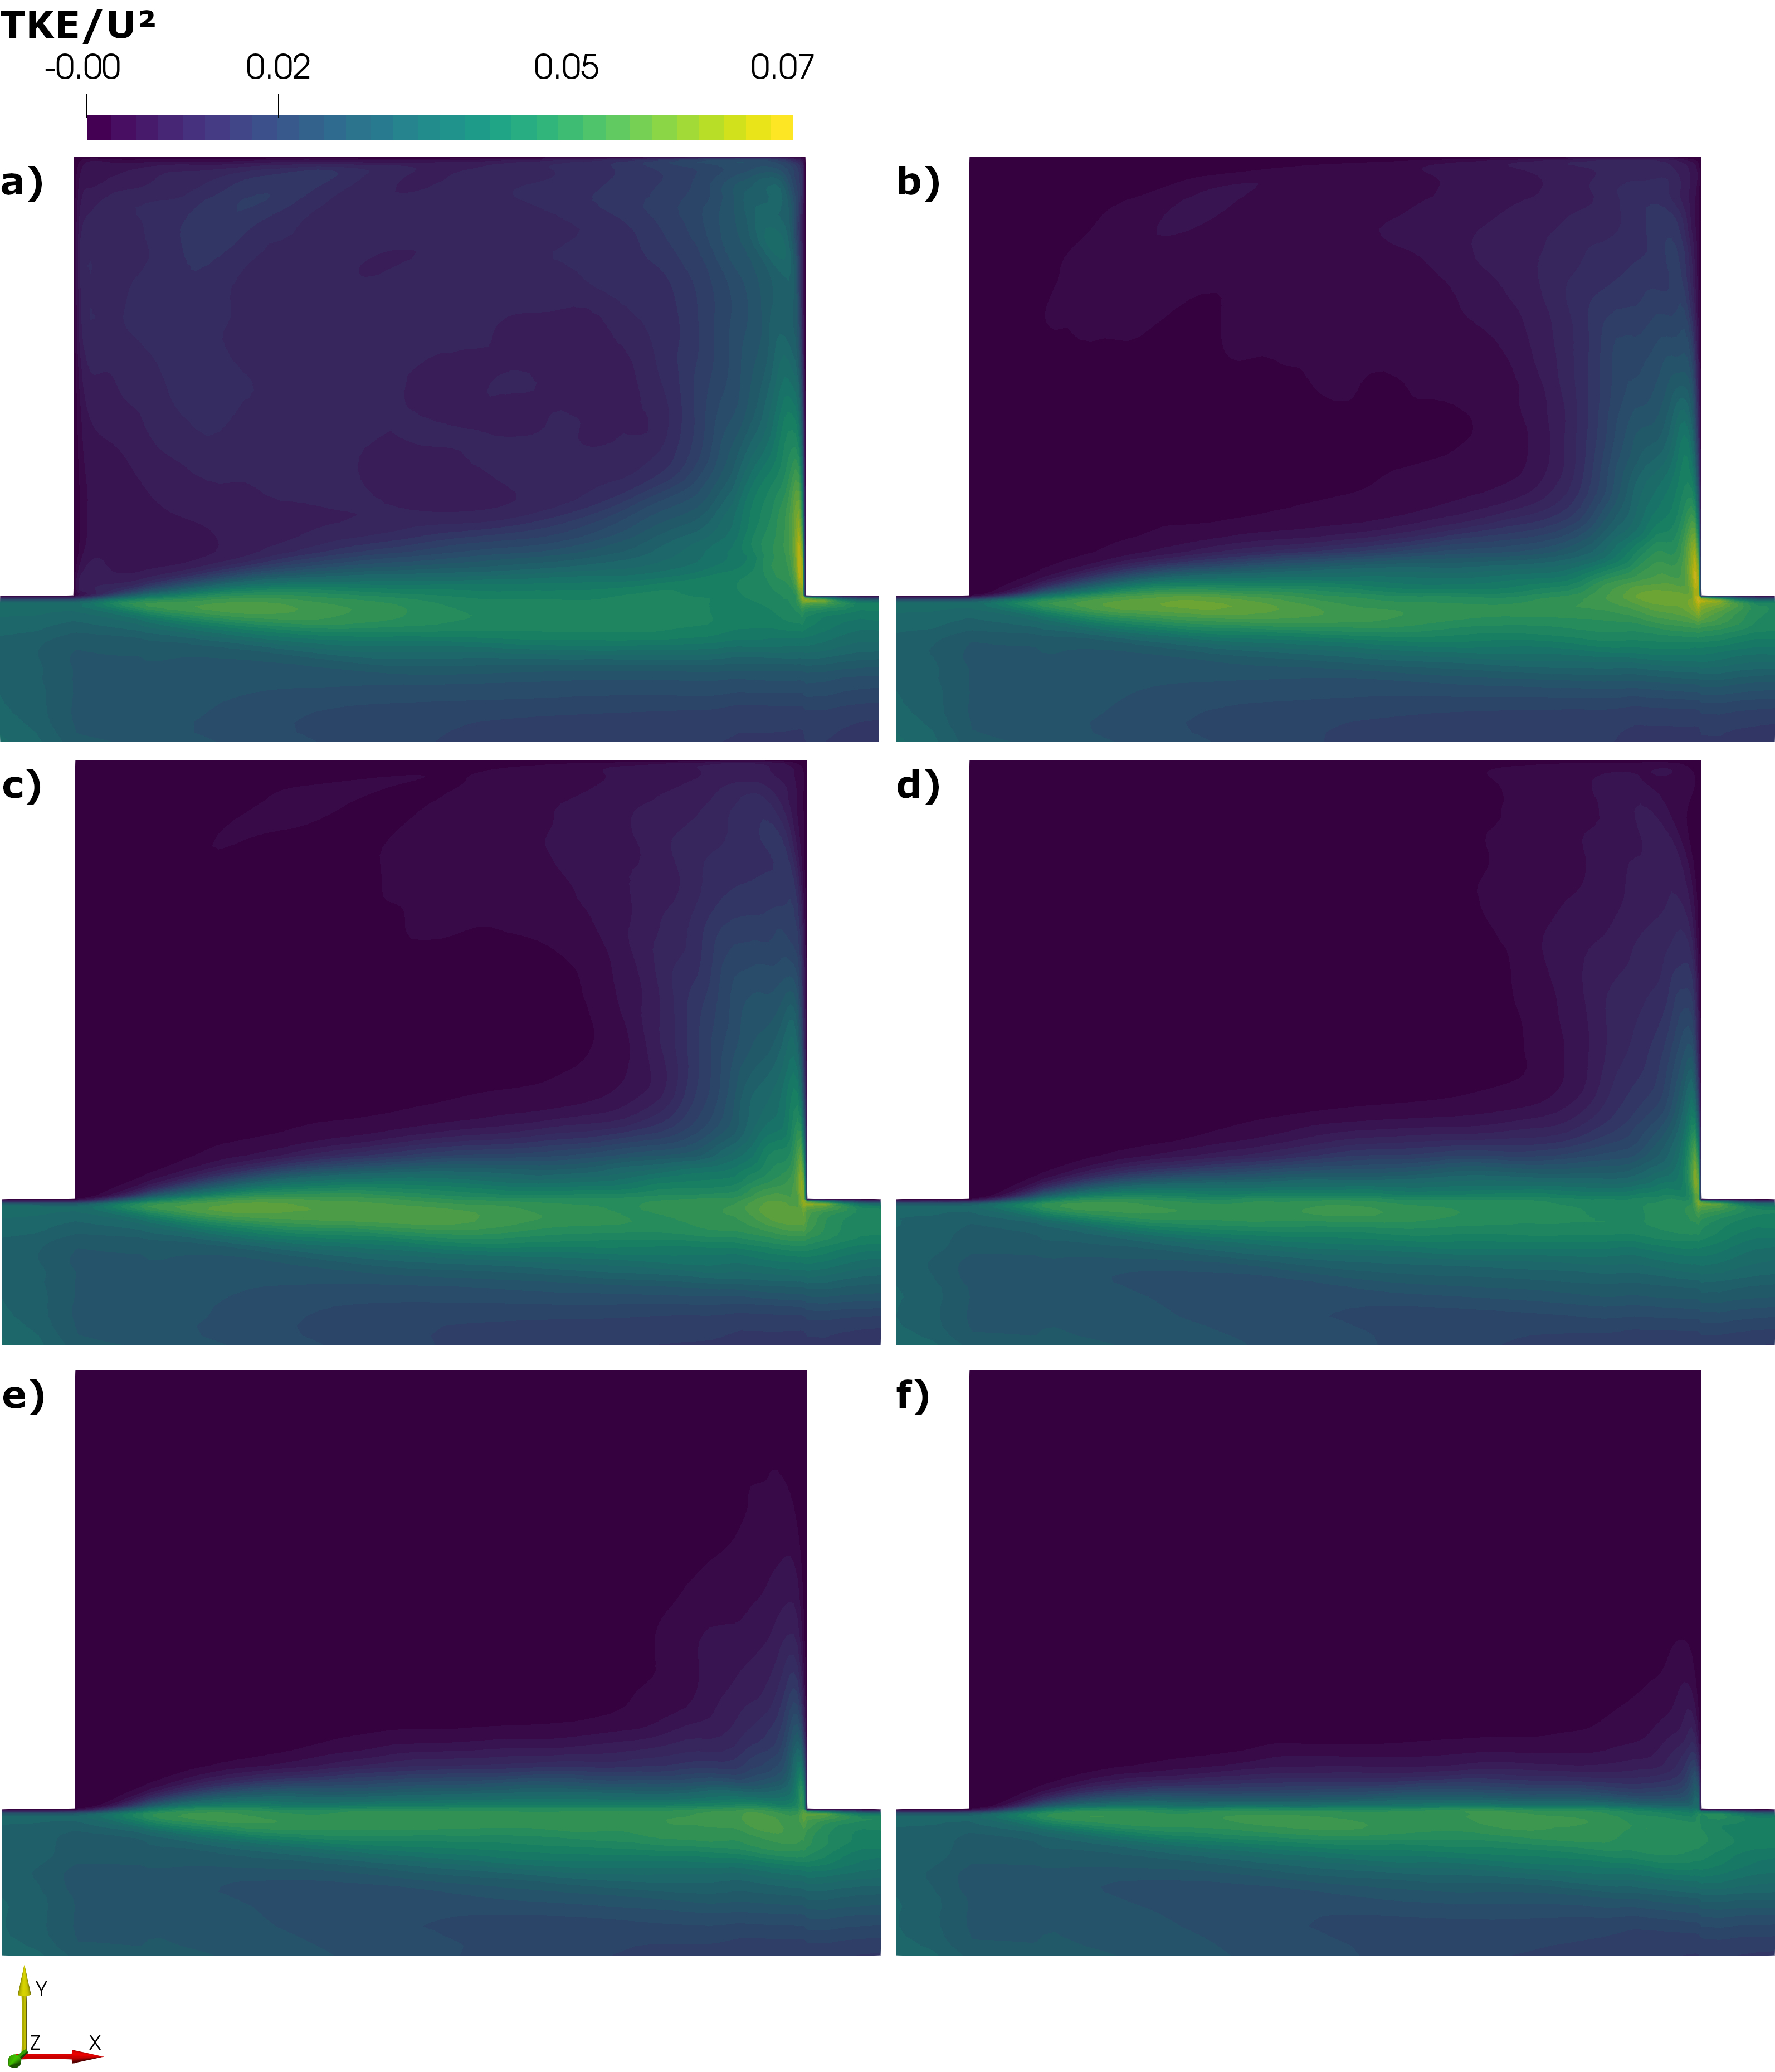
\includegraphics[width=\linewidth]{../images/art4/totalTKEMean1.jpeg}
\caption{Time-averaged total kinetic energy (TKE) at z/h = 0.6: a) Case 0, b) Case 1, c) Case 2, d) Case 3, e) Case 4 and f) Case 5.}
\label{fig:art4:totalTKEMean1}
\end{figure}

\begin{figure}[!ht]
\centering
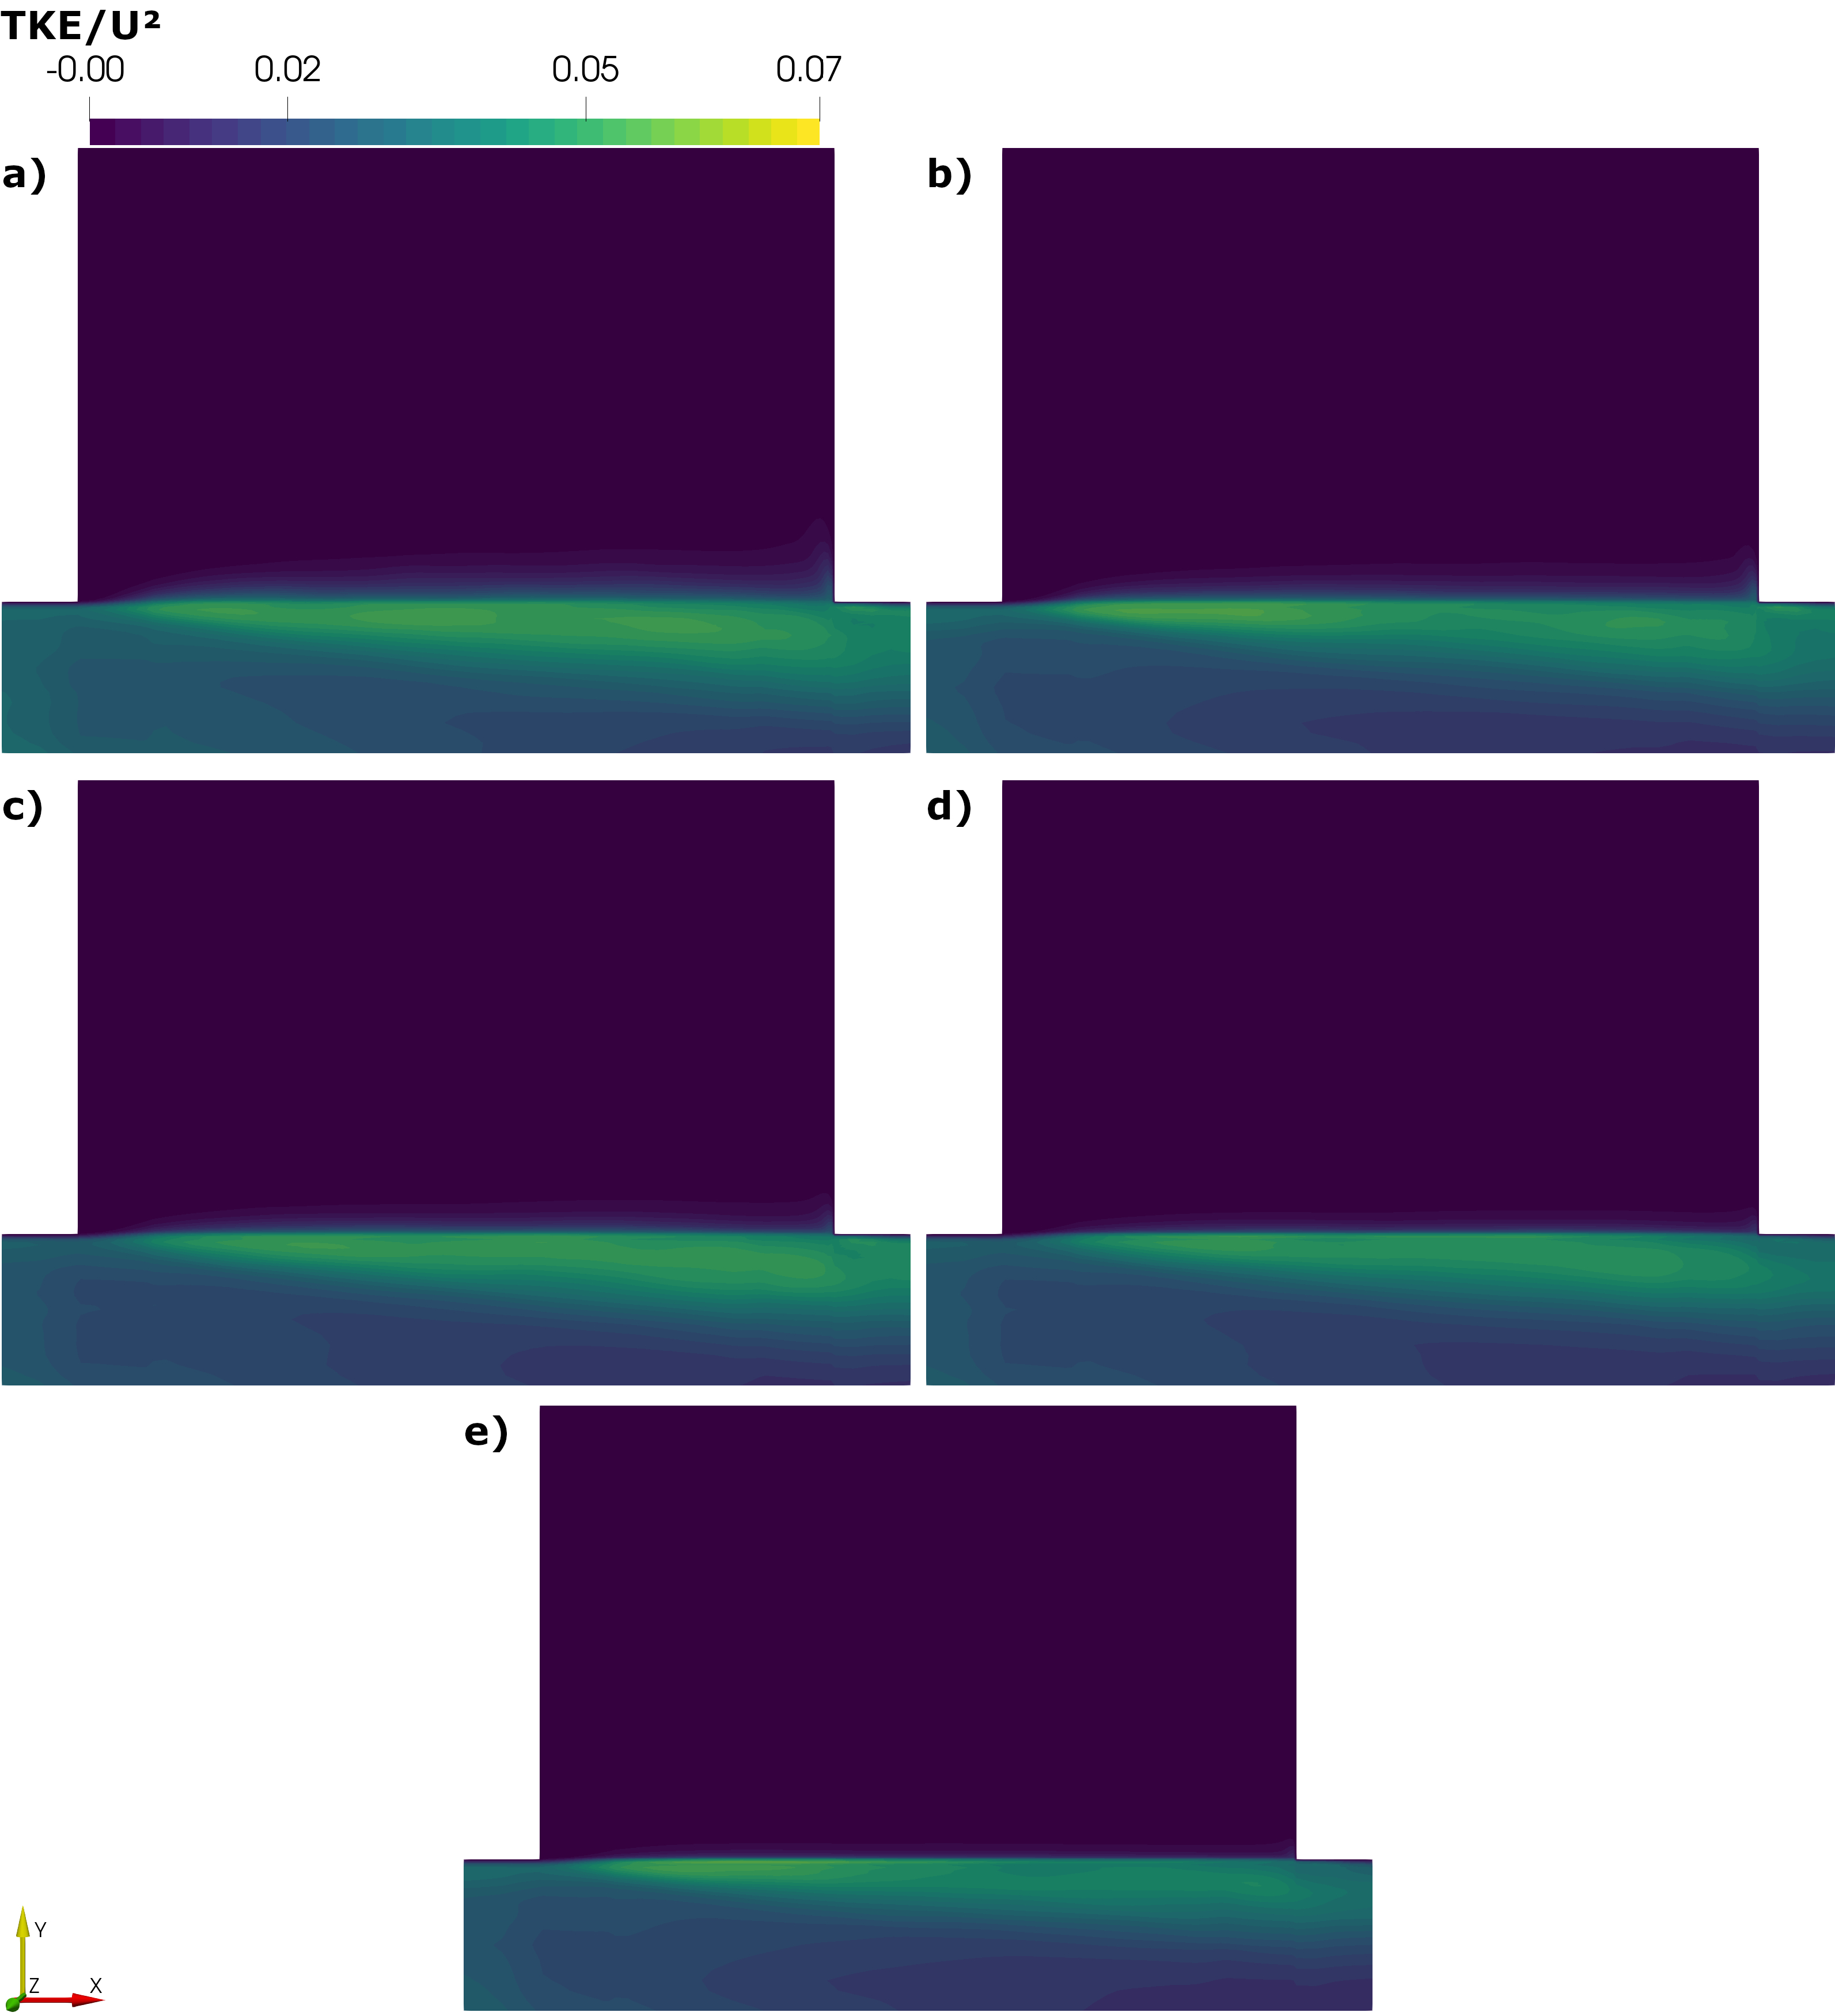
\includegraphics[width=\linewidth]{../images/art4/totalTKEMean2.jpeg}
\caption{Time-averaged total kinetic energy (TKE) at z/h = 0.6: a) Case 6, b) Case 7, c) Case 8, d) Case 9 and e) Case 10.}
\label{fig:art4:totalTKEMean2}
\end{figure}

\section{Mass Exchange}
The mass exchange coefficient $k$ is an important parameter of the cavity, as one of its main characteristics is the transient storage of mass. This coefficient indicates the mass exchange rate between the cavity and the main channel. The evaluation of this parameter through tracer experiments was done using a first-order exponential decay in which the initial concentration was set to 1. Analogously, the mean retention time ($T_{cav}$) is the time needed to completely replace the water volume in the cavity. This parameter was adjusted using a non-linear least square method to best approximate the value of $T_{cav}$ to the volumetric-average tracer concentration through time \cite{weitbrecht2004} (Figure \ref{fig:art4:massConcentration}).

\begin{equation}
C=C_0 e^{-t/T_{cav}}
\label{eqn:art4:concentration}
\end{equation}

\begin{equation}
k=\frac{W}{T_{cav} U}
\label{eqn:art4:k}
\end{equation}

where, $C_0=1$ is the initial concentration, $t$ (s) is the time and $T_{cav}$ (s) is the mean retention time and $k$ is the mass exchange coefficient.

\begin{figure}[!ht]
\centering
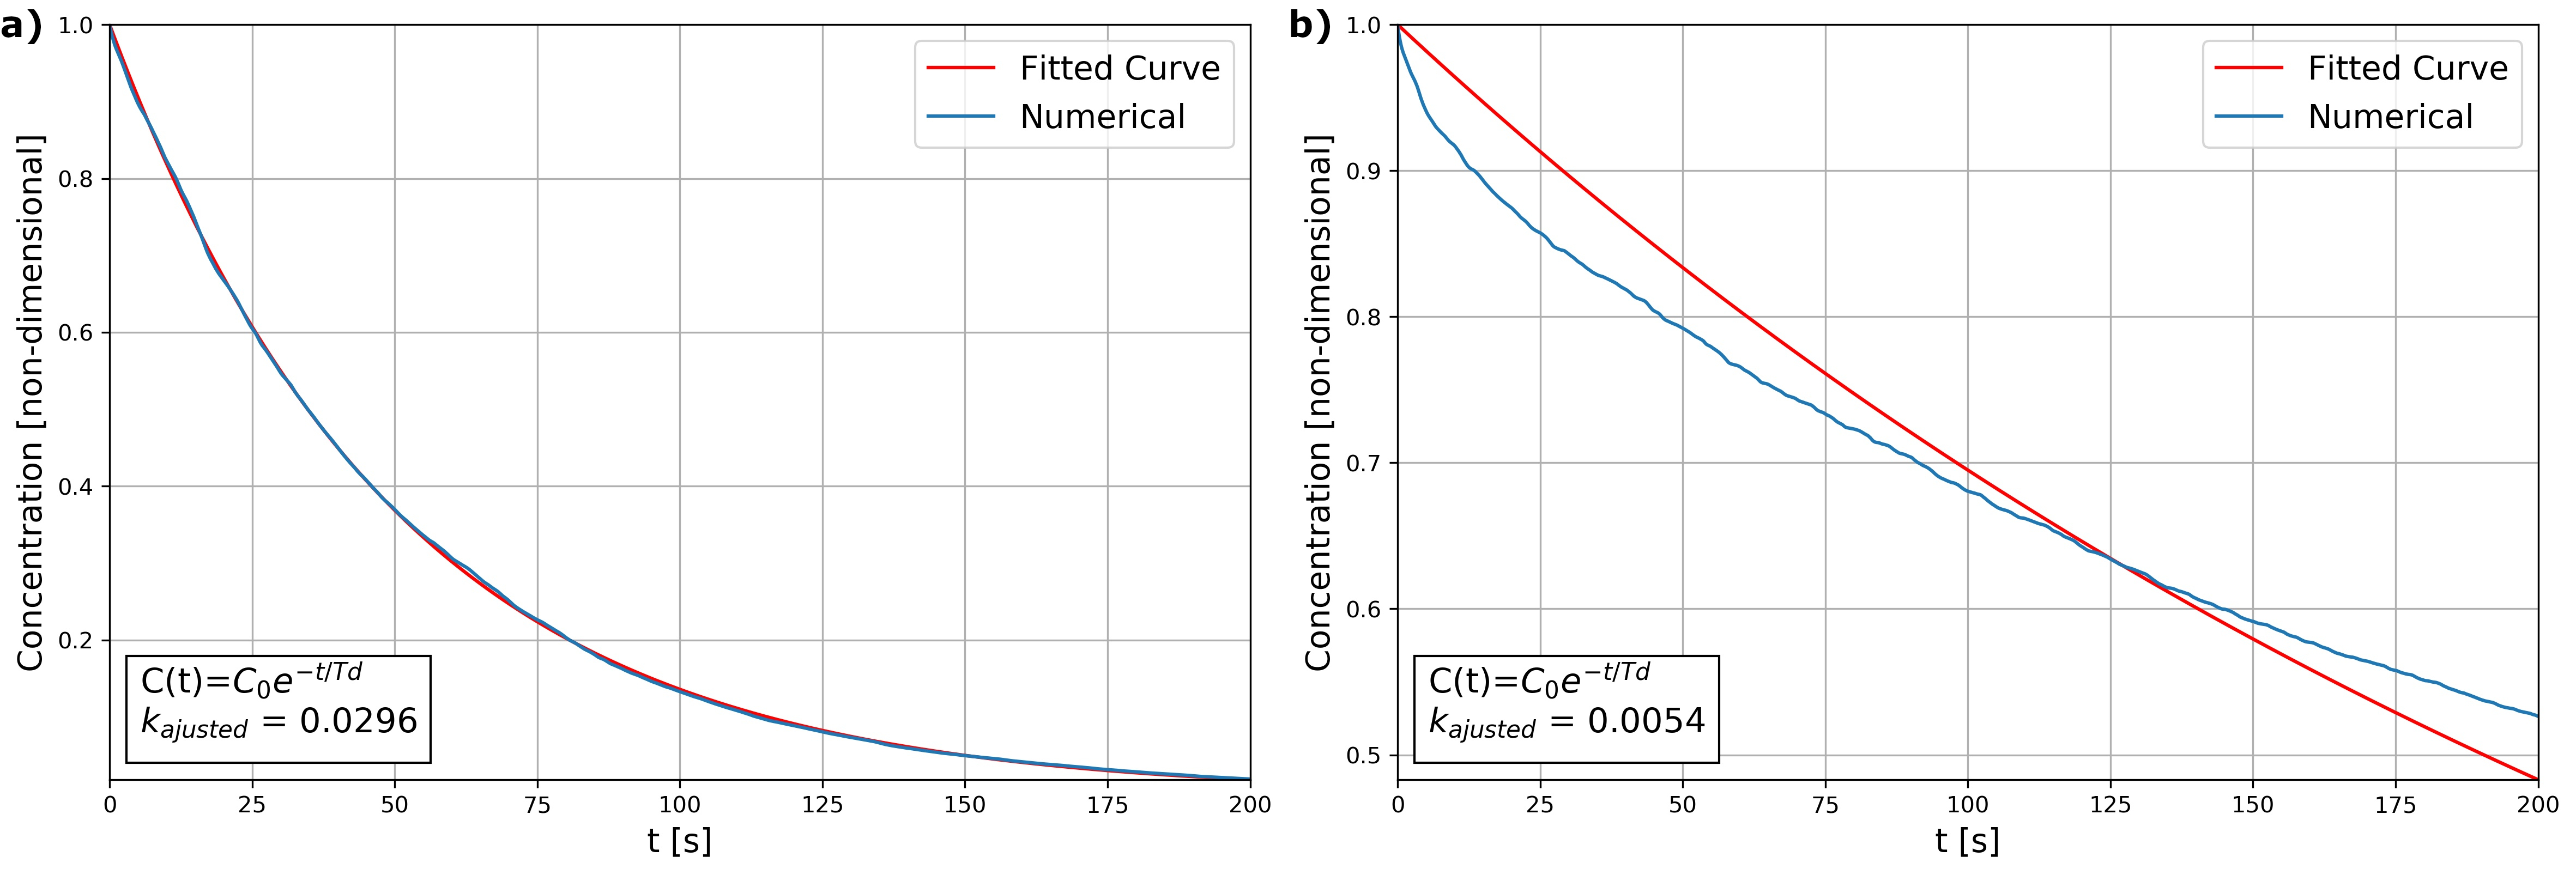
\includegraphics[width=\linewidth]{../images/art4/massDecay.jpeg}
\caption{Volumetric-averaged tracer concentration decay inside the lateral cavity over time: a) Case 1 b) Case 8.}
\label{fig:art4:massConcentration}
\end{figure}

Figure \ref{fig:art4:massExchange} shows the variation of the mass exchange coefficient and the mean retention time with the increase of vegetation density $a$. Analogous to \textcite{xiang2019}, the tracer fields indicated a deviation in the curve near $a \approx 0.33$ which is related first to the plant-induced Karman vortex street and Kelvin-Helmholtz eddies \cite{Nepf2012} which decreased the $k$ decay rate and second the vegetation blockage that becomes the main effect further that point. Further that point, the mass exchange coefficient decreases with the increase of vegetation density in two different phases divided at $a \approx 4$\%. It is possible to assume that this vegetation density acted as a wall as the flow cannot penetrate the cavity enough for the flow to occur, the remaining exchange occurred in a thin layer that further reduced its width as the density increased. The presence of the secondary circulation for $a \geq 5.3280$\% (Case 8) implied that a further increase in vegetation density could divide the secondary phase into a two slope section of the curve, where the first circulation ejects mass faster than the secondary with slower velocities and no contact with the main channel \cite{deOliveira2020} (Figure \ref{fig:art4:massConcentration} a and b).

\begin{figure}[!ht]
\centering
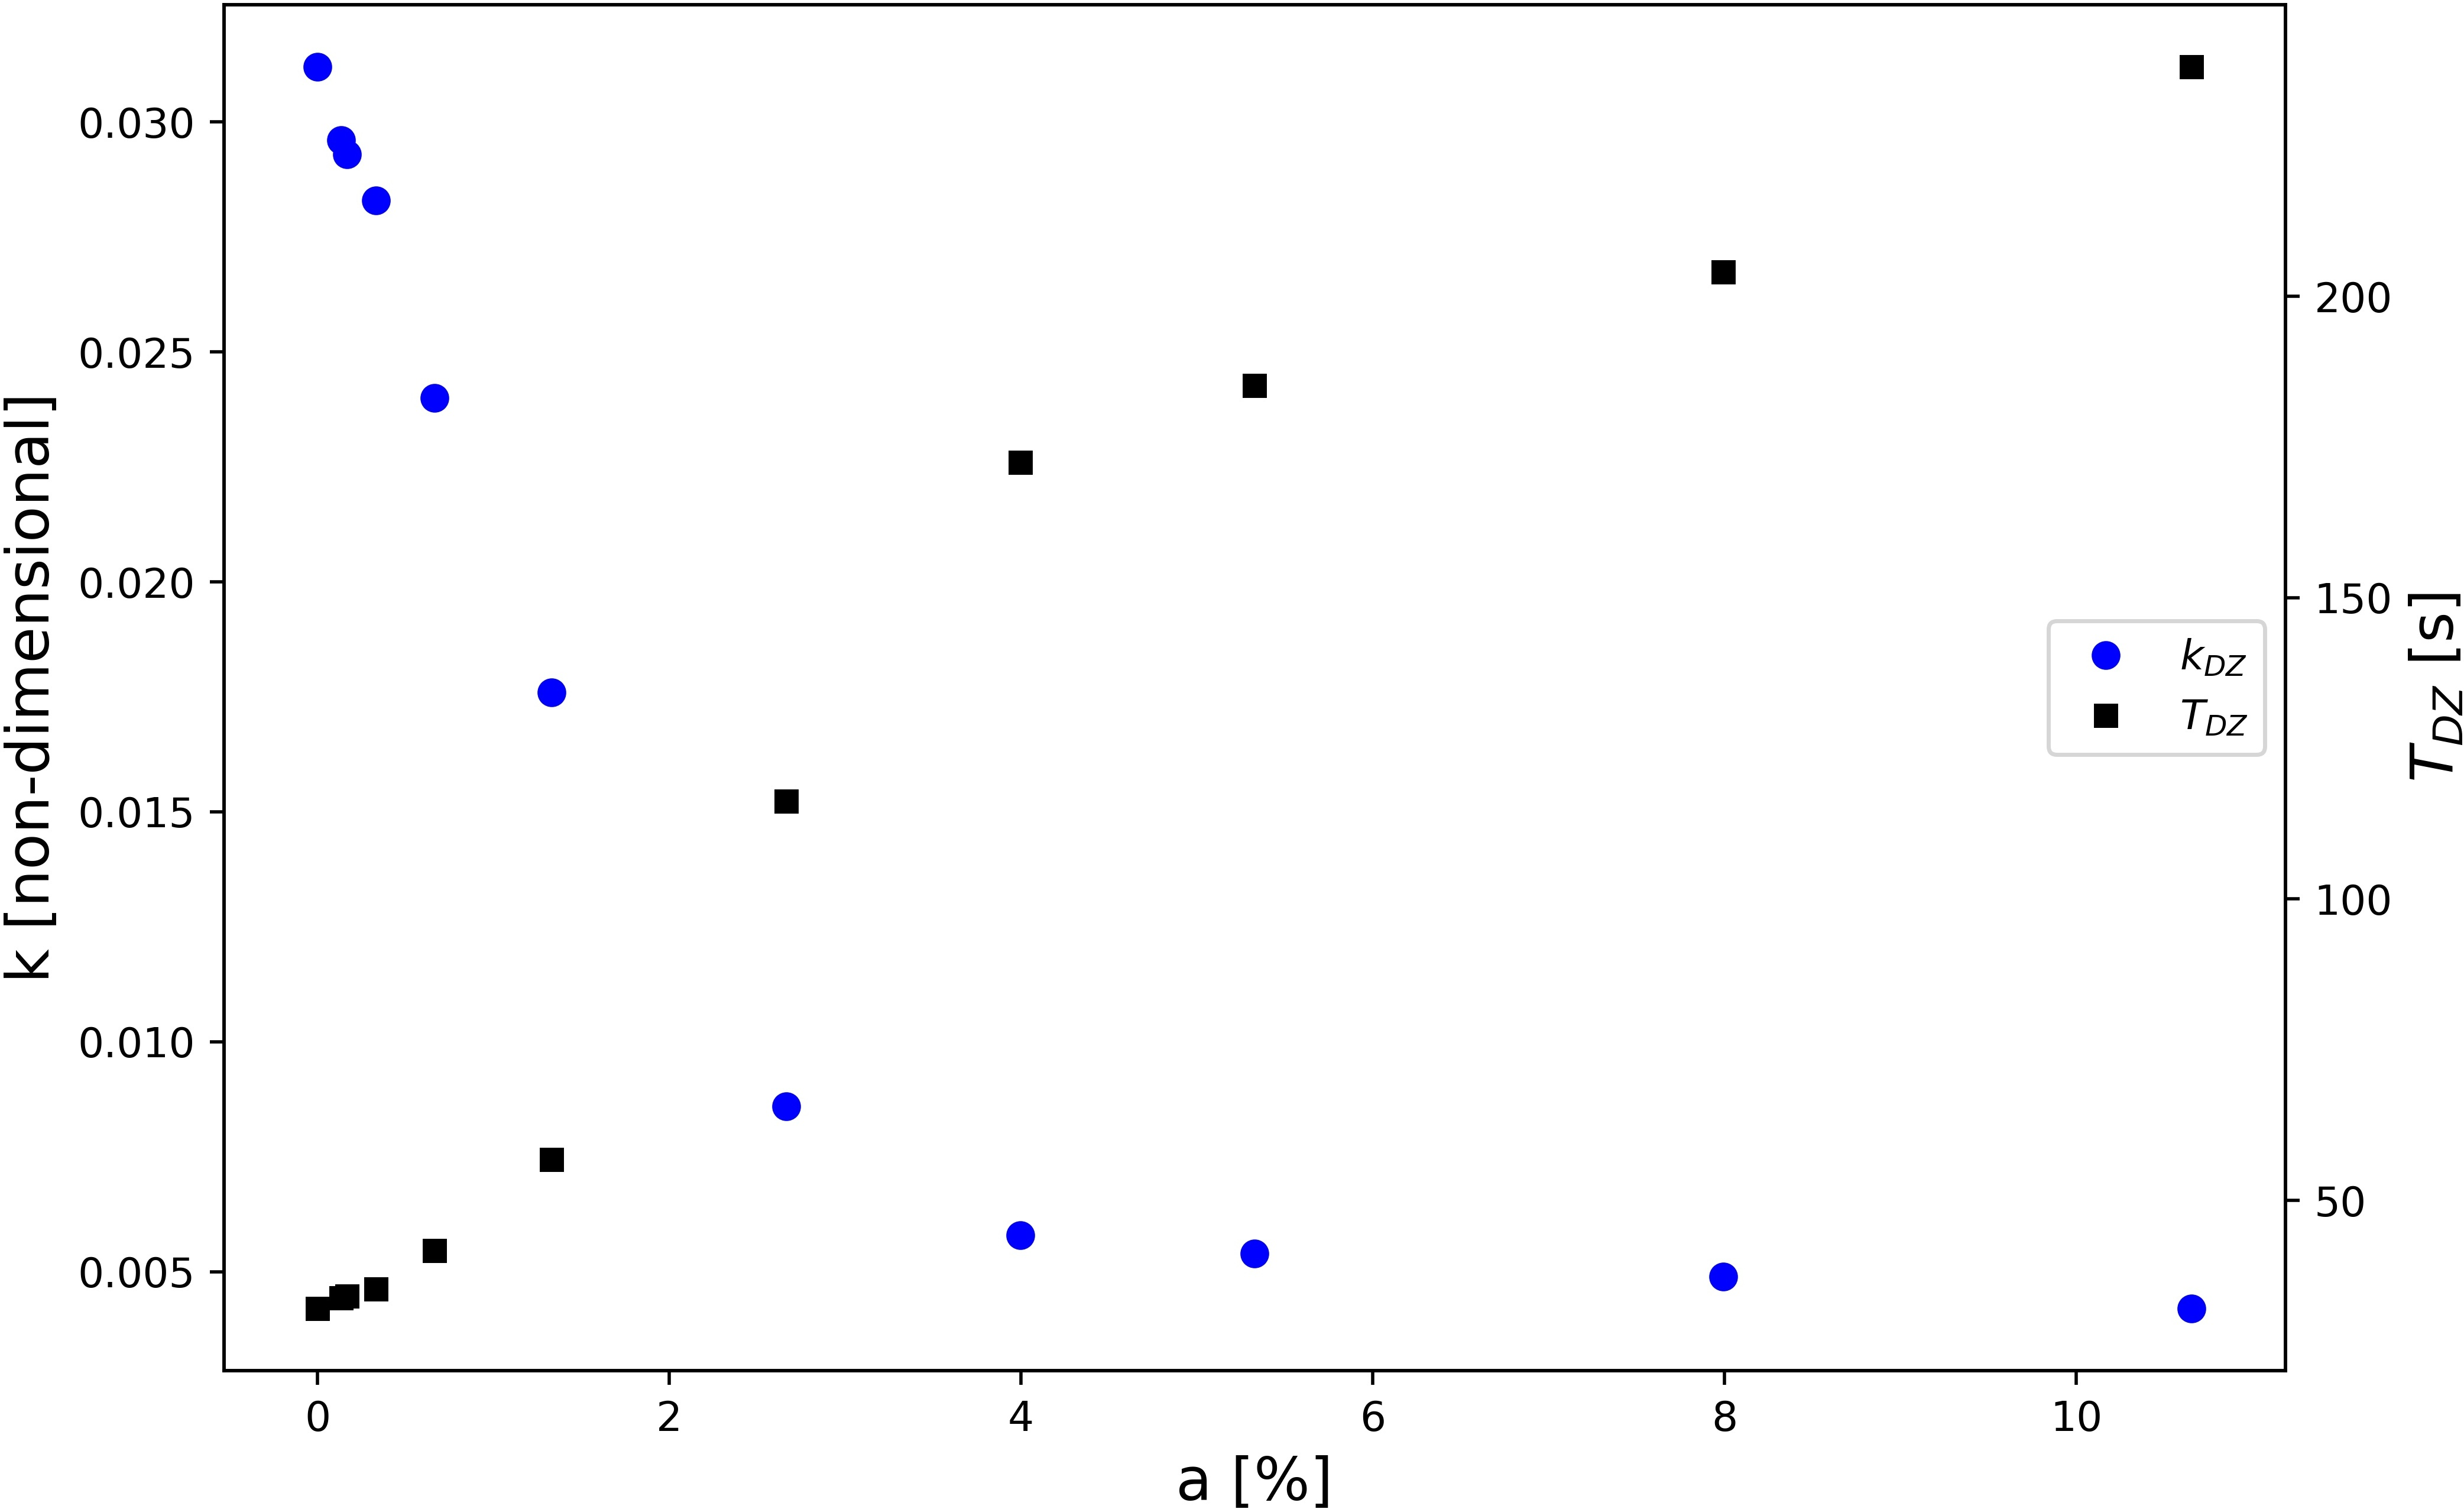
\includegraphics[width=\linewidth]{../images/art4/massExchange.jpg}
\caption{The variation of the mass exchange coefficient and the mean retention time with the increase of vegetation density.}
\label{fig:art4:massExchange}
\end{figure}

For low-vegetation density ($a < 4$\%), $k$ drops off quickly with increasing vegetation density $a$. For high-vegetation density ($a \geq 4$\%), $k$ is small, but not zero, and decreases slowly with increasing $a$. As the vegetation drag becomes the dominant effect, the velocity within the cavity becomes negligibly small, and it behaves as if the cavity is fully blocked ($\phi = 1$). The mass exchange, then, occurs mainly near the interface volume, this could be an influence of the increase of TKE in the outer part of the mixing layer. The effect of higher TKE levels in the outer mixing layer provides clear water volumes to scratch the vegetation at the interface. As the width of the TKE distribution decreases after a maximum at $a = 5.3380$ \%, the diminishing rate that clear water is available at the interface further slows down the exchange between the zones. Furthermore, the presence of vorticity for $a \leq 7.9920$ indicates that the small vortices could be moving tracer and promoting its diffusion particularly at the inner mixing layer. This behaviour contributed to the mass exchange and the lack of this phenomenon can be seen past $a \geq 7.9920$ when the mass exchange seems to change the asymptote of $k$ decay.

\section{Conclusion}
The hydrodynamics of a single lateral cavity with different vegetation densities was investigated numerically through LES. The results reveal that the single circulation system (non vegetated case) can be transformed into a two-gyre system with the increase of vegetation density. The influence of this secondary gyre decreased the rate in which the mass exchange coefficient diminished.

The dynamic of the flow was examined with both the vorticity and the turbulent kinetic energy (TKE) that both decreased in the downstream direction for all vegetation densities. For $a<2.6640$ \%, the downstream section of the mixing layer has higher values of both TKE and vorticity due to reduced inflow of the shed vortices in the cavity. For $a>2.6640$ \%, these higher values did not appear as the vegetation drag further increased, which is attributable to high blockage effect. The effect of these variables seems to play the dominant effect of the mass exchange in high-density vegetation, as the mass exchange mostly occurs at the inner mixing layer, region where these variables remain not null up to $a=5.3380$ \% for TKE and $a=7.9920$\% for vorticity.

This study enriched the knowledge of interactions between aquatic vegetation and the flow inside a lateral cavity. It shows that vegetation can drastically alter the flow by reducing the velocity, TKE and vorticity, this influence could promote the deposition of fine sediments and organic matter. Furthermore, it shows that the vegetation can cause a threshold in the mass exchange between the main channel and the lateral cavity, in which the rate is drastically reduced due to high blockage effects. This knowledge could help river managers to set limits and adjust the vegetation density inside the cavity in order to keep the desirable ecological function of the cavity.

\addcontentsline{toc}{section}{Funding}
\section*{Funding}
This study was financed in part by the Coordenação de Aperfeiçoamento de Pessoal de Nível Superior - Brazil (CAPES) -Finance Code 001.

This study was partly conducted in Lobo Carneiro cluster located in NACAD/Coppe - Rio de Janeiro, Brazil

\addcontentsline{toc}{section}{References}
\printbibliography[segment=\therefsegment,heading=subbibliography, title={References}]